%=========================================================
% SEMINAR REPORT
% REAL-TIME DETECTION METHOD FOR CRACKED EGGS BASED ON
% IMPROVED YOLOV8 AND DUAL VERIFICATION WITH TRIPLE
% CLASSIFICATION GRANULARITY
%=========================================================

\documentclass[12pt,a4paper]{report}
\usepackage[T1]{fontenc}
\usepackage[utf8]{inputenc}

%=========================================================
% PACKAGES
%=========================================================

\usepackage[a4paper,
            top=1in,
            bottom=1in,
            left=1.3in,
            right=1in]{geometry}

% PDFLaTeX-compatible Times-style font
\usepackage{newtxtext}
\usepackage{newtxmath}

\usepackage{graphicx}
\graphicspath{{./}{./figures/}}
\usepackage{fancyhdr}
\usepackage{titlesec}
\usepackage{tocloft}
\usepackage{setspace}
\usepackage{amsmath,amssymb}
\usepackage{enumitem}
\usepackage{hyperref}
\usepackage{array}
\usepackage{caption}
\usepackage{xcolor}
\usepackage{float}
\usepackage{ragged2e}
\usepackage[nottoc,notlof,notlot]{tocbibind}
\usepackage{longtable}
\usepackage{etoolbox}

% Remove 10pt inter-chapter vertical gaps in List of Figures and List of Tables
\makeatletter
\def\ttl@addvspace#1#2{}
\patchcmd{\@chapter}{\addtocontents{lof}{\protect\addvspace{10\p@}}}{}{}{}
\patchcmd{\@chapter}{\addtocontents{lot}{\protect\addvspace{10\p@}}}{}{}{}
\makeatother

%=========================================================
% HYPERLINK SETTINGS
%=========================================================

\hypersetup{
    colorlinks=true,
    linkcolor=black,
    citecolor=black,
    urlcolor=blue,
    pdftitle={REAL-TIME DETECTION METHOD FOR CRACKED EGGS BASED ON IMPROVED YOLOV8 AND DUAL VERIFICATION WITH TRIPLE CLASSIFICATION GRANULARITY},
    pdfauthor={Arjun Manoj}
}

%=========================================================
% GENERAL FORMATTING
%=========================================================

\onehalfspacing
\fontsize{12}{18}\selectfont

\setlength{\parindent}{0.5in}
\setlength{\parskip}{0pt}

%=========================================================
% CHAPTER FORMATTING
%=========================================================

\titleformat{\chapter}[display]
    {\normalfont\fontsize{16}{19}\selectfont\bfseries\centering}
    {\chaptertitlename\ \thechapter}
    {14pt}
    {\fontsize{16}{19}\selectfont\centering}

\titlespacing*{\chapter}
    {0pt}
    {-8pt}
    {14pt}

%=========================================================
% SECTION FORMATTING (EXACT 14PT)
%=========================================================

\titleformat{\section}
    {\normalfont\fontsize{14}{17}\selectfont\bfseries}
    {\thesection}
    {0.5em}
    {}

\titleformat{\subsection}
    {\normalfont\fontsize{14}{17}\selectfont\bfseries}
    {\thesubsection}
    {0.5em}
    {}

%=========================================================
% TABLE OF CONTENTS AND LIST FORMATTING
%=========================================================

\setlength{\cftbeforechapskip}{10pt}
\setlength{\cftbeforesecskip}{4pt}
\setlength{\cftbeforefigskip}{4pt}
\setlength{\cftbeforetabskip}{4pt}

\renewcommand{\cftchapfont}{\fontsize{12}{14}\selectfont\bfseries}
\renewcommand{\cftsecfont}{\fontsize{12}{14}\selectfont}

\renewcommand{\cftchappagefont}{\fontsize{12}{14}\selectfont\bfseries}
\renewcommand{\cftsecpagefont}{\fontsize{12}{14}\selectfont}

\setlength{\cftbeforetoctitleskip}{-0.5cm}
\setlength{\cftaftertoctitleskip}{0.8cm}

\renewcommand{\cfttoctitlefont}{\hfill\fontsize{24}{28}\selectfont\bfseries}
\renewcommand{\cftaftertoctitle}{\hfill}
\renewcommand{\cftloftitlefont}{\hfill\fontsize{24}{28}\selectfont\bfseries}
\renewcommand{\cftafterloftitle}{\hfill}
\renewcommand{\cftlottitlefont}{\hfill\fontsize{24}{28}\selectfont\bfseries}
\renewcommand{\cftafterlottitle}{\hfill}

%=========================================================
% HEADER AND FOOTER
%=========================================================

\pagestyle{fancy}

\fancyhf{}

\fancyhead[L]{
    \footnotesize College of Engineering, Cherthala
}

\fancyhead[R]{
    \footnotesize\leftmark
}

\fancyfoot[L]{
    \small Department of Computer Science and Engineering
}

\fancyfoot[R]{
    \small\thepage
}

\renewcommand{\headrulewidth}{0.4pt}
\renewcommand{\footrulewidth}{0.4pt}

\renewcommand{\chaptermark}[1]{
    \markboth{#1}{}
}

%=========================================================
% PLAIN PAGE STYLE
%=========================================================

\fancypagestyle{plain}{
    \fancyhf{}

    \fancyfoot[L]{
        \small Department of Computer Science and Engineering
    }

    \fancyfoot[R]{
        \small\thepage
    }

    \renewcommand{\headrulewidth}{0pt}
    \renewcommand{\footrulewidth}{0.4pt}
}

%=========================================================
% FIGURE AND TABLE CAPTION FORMAT
%=========================================================

\captionsetup[figure]{
    font=normalsize,
    labelfont=normalfont,
    justification=centering,
    singlelinecheck=true
}

\captionsetup[table]{
    font=normalsize,
    labelfont=bf,
    justification=centering,
    singlelinecheck=true
}

%=========================================================
% DOCUMENT INFORMATION
%=========================================================

\newcommand{\reporttitle}{REAL-TIME DETECTION METHOD FOR CRACKED EGGS BASED ON IMPROVED YOLOV8 AND DUAL VERIFICATION WITH TRIPLE CLASSIFICATION GRANULARITY}
\newcommand{\studentname}{ARJUN MANOJ}
\newcommand{\rollno}{CEC23CS043}
\newcommand{\guidename}{Mrs. NANDANA RAJ R}
\newcommand{\seminarmonth}{SEPTEMBER 2026}
\newcommand{\coordinator}{Mrs. Deepa C G}
\newcommand{\hodname}{Dr. Preetha Theresa Joy}
\newcommand{\principalname}{Dr. Jaya VL}

%=========================================================
% DOCUMENT
%=========================================================

\begin{document}

%=========================================================
% COVER PAGE (FIRST TITLE PAGE)
%=========================================================

\begin{titlepage}
\thispagestyle{empty}
\begin{center}

\vspace*{0.3cm}

{\Large\bfseries A SEMINAR REPORT ON}\par

\vspace{0.6cm}

{\fontsize{15}{21}\selectfont\bfseries
REAL-TIME DETECTION METHOD FOR CRACKED EGGS\\
BASED ON IMPROVED YOLOV8 AND DUAL\\
VERIFICATION WITH TRIPLE\\
CLASSIFICATION GRANULARITY\\}\par

\vspace{0.8cm}

{\large\itshape Submitted By}\par
\vspace{0.2cm}
{\large\bfseries\itshape \studentname\ (\rollno)}\par

\vspace{0.6cm}

{\large\itshape under the esteemed guidance of}\par
\vspace{0.2cm}
{\large\bfseries\itshape \guidename}\par
\vspace{0.1cm}
{\large\itshape (Assistant Professor)}\par
\vspace{0.15cm}
{\large\itshape Department of Computer Science and Engineering}\par

\vfill


\includegraphics[width=3.2cm]{logo.jpg}\par

\vfill

{\large\bfseries \seminarmonth}\par
\vspace{0.05cm}
{\large\bfseries DEPARTMENT OF COMPUTER SCIENCE AND ENGINEERING}\par
{\large\bfseries COLLEGE OF ENGINEERING, PALLIPPURAM P O, CHERTHALA,}\par
{\large\bfseries ALAPPUZHA PIN: 688541,}\par
{\large\bfseries PHONE: 0478 2553416, FAX: 0478 2552714}\par
{\large\bfseries http://www.cectl.ac.in}\par

\vspace*{0.2cm}
\end{center}
\end{titlepage}

%=========================================================
% SECOND TITLE PAGE
%=========================================================

\begin{titlepage}
\thispagestyle{empty}
\begin{center}

\vspace*{0.2cm}

{\Large\bfseries A SEMINAR REPORT ON}\par

\vspace{0.45cm}

{\fontsize{15}{21}\selectfont\bfseries
REAL-TIME DETECTION METHOD FOR CRACKED EGGS\\
BASED ON IMPROVED YOLOV8 AND DUAL\\
VERIFICATION WITH TRIPLE\\
CLASSIFICATION GRANULARITY\\}\par

\vspace{0.5cm}

{\large\itshape Submitted By}\par
\vspace{0.15cm}
{\large\bfseries\itshape \studentname\ (\rollno)}\par

\vspace{0.35cm}

{\large\itshape under the esteemed guidance of}\par
\vspace{0.15cm}
{\large\bfseries\itshape \guidename}\par
\vspace{0.1cm}
{\large\itshape (Assistant Professor)}\par

\vspace{0.35cm}

{\large\itshape In partial fulfillment of the requirements for the award of the degree}\par
{\large\itshape of}\par
{\large\bfseries Bachelor of Technology}\par
{\large\itshape in}\par
{\large\bfseries Computer Science and Engineering}\par
{\large\itshape of}\par
{\large\bfseries APJ Abdul Kalam Technological University}\par

\vfill


\includegraphics[width=3.0cm]{logo.jpg}\par

\vfill

{\large\bfseries \seminarmonth}\par
\vspace{0.05cm}
{\large\bfseries DEPARTMENT OF COMPUTER SCIENCE AND ENGINEERING}\par
{\large\bfseries COLLEGE OF ENGINEERING, PALLIPPURAM P O, CHERTHALA,}\par
{\large\bfseries ALAPPUZHA PIN: 688541,}\par
{\large\bfseries PHONE: 0478 2553416, FAX: 0478 2552714}\par
{\large\bfseries http://www.cectl.ac.in}\par

\vspace*{0.2cm}
\end{center}
\end{titlepage}

%=========================================================
% CERTIFICATE PAGE
%=========================================================

\thispagestyle{empty}
\begin{center}
{\large\bfseries DEPARTMENT OF COMPUTER SCIENCE AND ENGINEERING}\par
{\large\bfseries COLLEGE OF ENGINEERING CHERTHALA}\par
{\large\bfseries ALAPPUZHA-688541}\par
\vspace{0.3cm}

\includegraphics[width=2.8cm]{logo.jpg}\par
\vspace{0.3cm}
{\Large\bfseries C E R T I F I C A T E}\par
\end{center}

\vspace{0.4cm}
\noindent
This is to certify that, the seminar report titled \textbf{\textit{\reporttitle}} is a bonafide record of the \textbf{CSQ413 SEMINAR} presented by \textbf{\studentname\ (\rollno)}, Seventh Semester B.Tech. Computer Science \& Engineering student, under our guidance and supervision, in partial fulfillment of the requirements for the award of the degree B.Tech. Computer Science \& Engineering of APJ Abdul Kalam Technological University.

\vspace{3.75cm}
\begin{center}
\begin{tabular}{@{}c@{\hspace{0.4cm}}c@{\hspace{0.4cm}}c@{}}
\textbf{Guide} & \textbf{Co-ordinator} & \textbf{HoD}\\[1.6cm]

\guidename & \coordinator & \hodname\\[0.15cm]

Assistant Professor & Assistant Professor & Professor\\[0.15cm]

\parbox[t]{5cm}{\centering Dept. of Computer Science\\\& Engineering} &
\parbox[t]{5cm}{\centering Dept. of Computer Science\\\& Engineering} &
\parbox[t]{5cm}{\centering Dept. of Computer Science\\\& Engineering}

\end{tabular}
\end{center}

\newpage

%=========================================================
% ACKNOWLEDGEMENT
%=========================================================

\pagenumbering{roman}
\setcounter{page}{1}

\chapter*{ACKNOWLEDGEMENT}
This seminar work would not have been possible without the support and encouragement of many people. First and foremost, I give thanks to Almighty God who gave me the strength, resources and ability to complete the seminar successfully.

I would like to express my sincere gratitude to our Principal, \textbf{\principalname}, for providing the necessary facilities and support for the completion and presentation of this seminar.

I am also deeply grateful to the Head of the Department, \textbf{\hodname}, for her encouragement and support throughout the seminar work.

I extend my heartfelt thanks to our seminar co-ordinators, \textbf{Mrs.~Deepa~C~G}, Assistant Professor, Department of Computer Science and Engineering, \textbf{Mrs.~Seethamol~S}, Assistant Professor, Department of Computer Science and Engineering and \textbf{Mrs.~Vidya~S~Mony}, Assistant Professor, Department of Computer Science and Engineering for their valuable coordination and guidance. I am especially grateful to my guide, \textbf{\guidename}, Assistant Professor, Department of Computer Science and Engineering, for her constant guidance, encouragement and constructive suggestions throughout this seminar.

I would also like to thank my dear friends for their cooperation and encouragement throughout the seminar. Their support and understanding made the completion of this work easier and more meaningful.

\newpage

%=========================================================
% ABSTRACT
%=========================================================

\chapter*{ABSTRACT}

Eggshell integrity is a vital commercial quality indicator in the poultry processing industry. Approximately 3\% of fresh eggs suffer shell damage during production, handling, packaging and transit. Defective shells facilitate rapid bacterial penetration by pathogens such as \textit{Salmonella}, lead to internal moisture loss, cause liquid leakage and inflict substantial financial losses on poultry producers. Conventional sorting relies heavily on manual visual inspection, which is labor-intensive, subjective and vulnerable to worker visual fatigue. Non-destructive acoustic and traditional vision techniques struggle on dynamic conveyor lines due to factory acoustic noise, fluctuating illumination and natural dirt on unwashed eggs. Furthermore, conventional conveyors lack egg rotation mechanisms, leaving bottom surfaces uninspected.

This seminar presents an industrial-grade, real-time online detection method for cracked eggs based on an improved YOLOv8 framework and a dual verification mechanism with triple classification granularity. The mechanical conveying system integrates motor-driven rotating rollers across six parallel channels (360 eggs/minute throughput), rotating eggs through 360 degrees beneath an industrial CCD camera and uniform LED lighting box. Instead of binary classification, the framework introduces triple classification granularity: Category 1 (Intact Egg), Category 2 (Cracked Egg) and Category 3 (Crack Region). A redundant dual verification rule identifies an egg as damaged whenever either the overall cracked egg or localized crack region detector fires.

At the network architectural level, the baseline YOLOv8 model is structurally optimized for irregular hairline cracks. Deformable Convolution v2 (DCNv2) modules are integrated into the backbone to adapt receptive field shapes to jagged crack paths. A Weighted Bidirectional Feature Pyramid Network (BiFPN) replaces the standard PANet neck for multi-scale feature fusion. A dedicated P2 small target detection head operating on a $160 \times 160$ feature map is introduced to preserve micro-crack cues, while the Wise-IoU v2 (WIoUv2) loss function dynamically balances gradients across bounding box candidates. Experimental evaluations demonstrate that the improved YOLOv8 model achieves an mAP@0.5 of 92.9\% on the test set, representing a 5.2\% improvement over baseline YOLOv8 and outperforming Faster R-CNN, YOLOv5 and YOLOv11. On an industrial egg conveyor, the deployed system operates at 45 frames per second with an intact egg false alarm rate of 2.18\% and a compound broken egg miss rate of only 1.06\%, fully meeting industrial online grading criteria.

\clearpage

%=========================================================
% TABLE OF CONTENTS
%=========================================================

\tableofcontents

\clearpage

%=========================================================
% LIST OF FIGURES
%=========================================================

\clearpage
\markboth{List of Figures}{}
\thispagestyle{fancy}

\vspace*{-0.5cm}
{\centering\fontsize{24}{28}\selectfont\bfseries List of Figures\par}
\vspace{0.8cm}

\makeatletter
\l@figure{\numberline{2.1}{Structural schematic and operational overview of the egg conveying device}}{\pageref{fig:conveyor_device}}
\l@figure{\numberline{2.2}{Machine vision system architecture and industrial camera installation}}{\pageref{fig:vision_system}}
\l@figure{\numberline{2.3}{Triple classification granularity scheme: Intact Egg, Cracked Egg and Crack Region}}{\pageref{fig:categories}}
\l@figure{\numberline{2.4}{Detailed architectural layout of the improved YOLOv8 framework}}{\pageref{fig:yolov8_arch}}
\l@figure{\numberline{2.5}{Comparison of regular convolution sampling and DCNv2 deformable sampling on irregular cracks}}{\pageref{fig:dcnv2_sampling}}
\l@figure{\numberline{2.6}{Architectural comparison of multi-scale feature fusion structures: FPN, PANet and BiFPN}}{\pageref{fig:bifpn_structure}}
\l@figure{\numberline{2.7}{Comprehensive technical workflow spanning offline training, model export and online inference}}{\pageref{fig:training_schematic}}
\l@figure{\numberline{3.1}{Precision-Recall curves comparison between baseline YOLOv8 and the proposed model across all target categories}}{\pageref{fig:pr_curves}}
\l@figure{\numberline{3.2}{Visual detection comparisons of Faster R-CNN, YOLOv5, baseline YOLOv8 and the proposed improved model on unwashed eggs}}{\pageref{fig:visual_detection}}
\l@figure{\numberline{3.3}{Online deployment and testing on the industrial egg conveyor line}}{\pageref{fig:online_deployment}}
\l@figure{\numberline{3.4}{Visual detection results on active industrial conveyor with rotating eggs}}{\pageref{fig:production_detection}}
\l@figure{\numberline{3.5}{Online detection speed stability curve across 400 continuous frames at 45 FPS}}{\pageref{fig:online_speed}}
\makeatother

\clearpage

%=========================================================
% LIST OF TABLES
%=========================================================

\clearpage
\markboth{List of Tables}{}
\thispagestyle{fancy}

\vspace*{-0.5cm}
{\centering\fontsize{24}{28}\selectfont\bfseries List of Tables\par}
\vspace{0.8cm}

\makeatletter
\l@table{\numberline{1.1}{Summary of related research in automated egg defect inspection}}{\pageref{tab:literature_survey}}
\l@table{\numberline{2.1}{Dataset composition across partitions and defect categories}}{\pageref{tab:dataset_distribution}}
\l@table{\numberline{2.2}{Computational hardware specifications and software environment}}{\pageref{tab:hardware_software}}
\l@table{\numberline{3.1}{Ablation experiment results on test dataset}}{\pageref{tab:ablation_results}}
\l@table{\numberline{3.2}{Model complexity and computational footprint comparison}}{\pageref{tab:model_complexity}}
\l@table{\numberline{3.3}{Comparative performance benchmark across mainstream detectors}}{\pageref{tab:benchmark_comparison}}
\l@table{\numberline{3.4}{Online factory inspection error rates across 106 production video frames}}{\pageref{tab:online_inspection_errors}}
\makeatother

\clearpage

%=========================================================
% MAIN CONTENT
%=========================================================

\pagenumbering{arabic}
\setcounter{page}{1}

%=========================================================
% CHAPTER 1: INTRODUCTION
%=========================================================

\chapter{Introduction}

\section{Background and Commercial Significance}

Table eggs represent one of the most widely consumed, nutrient-dense and economical sources of animal protein globally. With the growth of modern intensive poultry farming, egg production has expanded into an automated, high-throughput industrial sector. Modern commercial egg packaging facilities routinely process hundreds of thousands of eggs daily. In these high-capacity operations, preserving the physical integrity of the eggshell is of paramount importance to ensure food safety, extend product shelf life and protect commercial profitability.

The avian eggshell is a naturally engineered bioceramic composite structure composed predominantly of calcium carbonate (around 95\% to 97\% calcite crystal matrix) interwoven with an organic protein matrix and sealed by an outermost waxy cuticle layer. Despite possessing impressive mechanical compression strength along its major axis, the eggshell is inherently thin and brittle, making it susceptible to fracture when subjected to dynamic mechanical impacts, point stresses, vibrations and lateral compression during gathering, packing and transit.

Maintaining shell integrity constitutes the primary biological barrier preventing external microorganisms from invading the nutrient-rich interior of the egg. When the structural continuity of the shell is compromised, the commercial and hygienic value of the egg declines drastically. Developing fast, automated and non-destructive quality evaluation systems capable of detecting shell defects in real time has emerged as an urgent priority for modern agricultural engineering.

\section{Eggshell Integrity and Breakage Challenges}

Across commercial egg production and distribution pipelines, empirical surveys indicate that approximately 3\% of all fresh eggs suffer shell breakage prior to retail delivery. While this percentage may appear modest in isolation, its cumulative impact across facilities processing hundreds of thousands of eggs per day translates into massive economic losses annually for industrial egg producers.

The consequences of cracked eggshells are severe:
\begin{enumerate}[label=\arabic*.]
    \item \textbf{Pathogen Infiltration and Food Safety Hazards:} A hairline fissure ruptures the physical protection provided by the shell and underlying testaceous membranes. This fissure provides an open entry corridor for environmental bacteria, including dangerous foodborne pathogens such as \textit{Salmonella enteritidis} and \textit{Escherichia coli}, presenting severe health risks to consumers.
    \item \textbf{Loss of Internal Freshness and Spoilage:} The crack accelerates evaporation of internal moisture and dissipation of carbon dioxide, thinning the thick albumen, flattening the yolk and precipitating premature spoilage.
    \item \textbf{Leakage and Secondary Batch Contamination:} In automated grading and packaging machinery, cracked eggs frequently rupture under mechanical handling. Liquid albumen and yolk leak onto conveyor rollers and surrounding intact eggs, fouling sorting machinery and contaminating entire batches of clean, marketable eggs.
\end{enumerate}

\section{Eggshell Morphology and Defect Manifestation}

Morphologically, the shell consists of the inner and outer testaceous membranes, the mammillary layer, the palisade layer of columnar calcite crystals, the vertical crystal layer and the protective waxy cuticle. While the palisade layer imparts high compressive strength, the brittle calcite matrix is vulnerable to flexural tensile stresses and fracture propagation under localized impacts.

Eggshell defects manifest in several morphologies:
\begin{itemize}
    \item \textbf{Hairline Micro-Cracks:} Fine, narrow fissures with widths under 0.1 mm penetrating the calcite layer. Due to their minute aperture, they produce minimal optical shadow and subtle gradient transitions.
    \item \textbf{Impact and Puncture Cracks:} Fractures caused by sharp point contact, featuring a central crushed indentation surrounded by radiating star-like micro-fissures.
    \item \textbf{Reticular Spider-Web Cracks:} Intricate networks of interconnected fine cracks covering broad areas of the egg equator.
\end{itemize}

A critical challenge in automated vision is distinguishing genuine hairline cracks from non-defective surface artifacts present on unwashed eggs, such as pigmentation speckles, dust particles, feather residues and dried manure streaks.

\section{Limitations of Existing Inspection Modalities}

Historically, the identification of defective eggs has relied on manual visual inspection (manual candling), where trained workers visually observe eggs rolling over an illuminated light table. However, manual candling exhibits severe operational bottlenecks: extreme visual fatigue leading to declining accuracy after 20 to 30 minutes, subjective assessment, high labor costs and an inability to keep pace with modern conveyors processing over 360 eggs per minute.

To eliminate dependence on human labor, automated non-destructive detection technologies have been investigated:
\begin{itemize}
    \item \textbf{Acoustic Resonance Methods:} Mechanical strikers tap the eggshell to capture acoustic vibrational response spectra. While effective in quiet laboratories, acoustic methods are vulnerable to severe ambient acoustic noise from factory conveyors and mechanical contact risks micro-fracturing thin shells.
    \item \textbf{Traditional Computer Vision:} Classical algorithms employ grayscale thresholding (Otsu binarization) and edge filters. However, these methods fail on unwashed eggs where natural dust, feathers and dried manure streaks generate false edges that confuse thresholding rules.
    \item \textbf{Existing Deep Learning Approaches:} Prior convolutional networks (such as Faster R-CNN) suffer from excessive latency ($\le 17$ FPS) that fails to meet production speeds ($\ge 30$ FPS). Crucially, existing vision rigs lack egg rotation mechanisms, capturing only a single perspective and leaving the underside shell surface uninspected.
\end{itemize}

\section{Literature Survey and Prior Work}

Automated quality inspection of eggshells has evolved through acoustic and optical processing techniques. Sun et al. (2020) investigated acoustic resonance inspection for hen and duck eggs using correlation analysis of impact sound waves. While intact shells displayed symmetric resonant peaks, factory background noise and the risk of striker damage limited industrial adoption. Balci et al. (2026) converted acoustic signals into spectrograms for CNN classification, yet acoustic interference from conveyor motors remained an obstacle.

In optical inspection, Liang et al. (2020) developed an integrated vision system utilizing histogram thresholding and Otsu segmentation on static egg images, achieving 98.18\% accuracy. However, hand-crafted thresholding failed on unwashed eggs where natural dirt, feathers and dried manure generated high-contrast edges, resulting in unacceptably high false alarm rates.

To improve defect feature extraction, Datta et al. (2019) applied Faster R-CNN with a ResNet backbone to chicken eggshells, achieving a 75\% mAP on severe cracks. Despite precise localization, the Region Proposal Network generated significant latency ($\approx 17$ FPS), falling short of industrial line speeds ($\ge 30$ FPS). Furthermore, the model struggled to resolve fine hairline cracks.

Turkoglu (2021) proposed a hybrid CNN-BiLSTM network for egg surface defect detection, attaining 96.3\% accuracy. Nevertheless, the sequential processing of recurrent LSTM units introduced computational bottlenecks that prevented high-speed parallel GPU inference on dynamic conveyor streams.

Botta et al. (2022) trained deep CNNs on static chicken egg images, reaching 95.38\% accuracy. However, their static imaging setup lacked egg rotation, leaving cracks on the bottom hemisphere entirely uninspected.

Yin et al. (2024) developed a lightweight YOLOv5l model with Ghost modules and ECA attention for cracked duck eggs, achieving 93.8\% accuracy. While efficient, their validation was limited to duck eggs, which possess thicker shells and higher contrast than chicken eggs. Furthermore, binary classification ignored localized crack regions.

Huang et al. (2023) tackled unwashed egg inspection using YOLOv5 with BiFPN and Coordinate Attention on video streams, achieving 96.4\% accuracy. However, their system lacked localized crack verification and full 360-degree rotation during transit, leaving underside defects undetected.

\section{Summary of Literature Survey}

Table~\ref{tab:literature_survey} summarizes prominent related studies in egg defect inspection, detailing methodologies, datasets, results and operational limitations.

\begin{table}[H]
\centering
\caption{Summary of related research in automated egg defect inspection}
\label{tab:literature_survey}
\vspace{0.2cm}
\setlength{\tabcolsep}{4pt}
\renewcommand{\arraystretch}{1.15}
\small
\begin{tabular}{|p{2.8cm}|p{2.6cm}|p{2.4cm}|p{1.8cm}|p{4.6cm}|}
\hline
\textbf{Study and Year} & \textbf{Methodology} & \textbf{Dataset} & \textbf{Result} & \textbf{Limitations} \\
\hline
Liang et al. (2020) & Otsu segmentation and thresholding & Static lab egg images & 98.18\% acc. & Sensitive to lighting; fails on unwashed surface dirt. \\
\hline
Datta et al. (2019) & Faster R-CNN with ResNet backbone & Static chicken eggshells & 75\% mAP & High computational cost; 17 FPS latency; misses hairline cracks. \\
\hline
Turkoglu (2021) & Hybrid CNN and Bidirectional LSTM & Egg surface defect dataset & 96.3\% acc. & Heavy parameter size; sequential recurrent latency limits speed. \\
\hline
Botta et al. (2022) & Deep Convolutional Neural Network & Static chicken egg images & 95.38\% acc. & Static setup; lacks egg rotation, leaving bottom uninspected. \\
\hline
Yin et al. (2024) & YOLOv5l with Ghost modules and ECA & Cracked duck egg dataset & 93.8\% acc. & Tested only on duck eggs; binary labeling misses micro-cracks. \\
\hline
Huang et al. (2023) & YOLOv5 with BiFPN and CA attention & Unwashed egg video streams & 96.4\% acc. & Lacks dual verification of localized crack zones; no rotation. \\
\hline
\end{tabular}
\end{table}

\section{Research Gap and Motivation}

A critical synthesis of the literature identifies key research gaps:
\begin{enumerate}[label=\arabic*.]
    \item \textbf{Absence of 360-Degree Rotation:} Static or non-rotating conveyors inspect only the upper hemisphere, creating severe blind spots on lateral and bottom shell surfaces.
    \item \textbf{Vulnerability to Natural Dirt:} Existing models trained on pre-washed supermarket eggs fail when exposed to dust, stains and manure on unwashed eggs.
    \item \textbf{Receptive Field Mismatch:} Rigid square kernels and aggressive downsampling in standard backbones dilute and obliterate sub-millimeter hairline cracks.
    \item \textbf{Coarse Binary Classification:} Single-label binary classification lacks redundancy, causing missed defective eggs when subtle cracks miss global thresholds.
    \item \textbf{Lack of Live Factory Validation:} Few studies evaluate real-time performance on industrial conveyor hardware operating at $\ge 30$ FPS.
\end{enumerate}

To overcome these limitations, this seminar investigates the improved YOLOv8 framework with dual verification and triple classification granularity formulated by Sun et al. (2026).

\section{Problem Statement}

Industrial egg processing facilities require an automated, real-time and non-destructive quality evaluation system capable of operating directly on high-speed conveyors carrying unwashed, moving eggs under actual factory conditions. The system must inspect the complete 360-degree surface of every egg to eliminate blind spots, operate at frame rates exceeding 30 frames per second (FPS) and maintain near-zero false negative rates for cracked eggs while minimizing false alarms on intact eggs carrying natural surface stains.

\section{Objectives}

The primary objective of this seminar study is to investigate, analyze and evaluate an industrial-grade, real-time cracked egg detection methodology based on an improved YOLOv8 architecture and a dual verification mechanism with triple classification granularity.

The specific objectives are:
\begin{enumerate}[label=\arabic*.]
    \item To examine a multi-channel conveying device with rotating rollers that enables complete 360-degree surface image acquisition without blind spots.
    \item To analyze the construction of an industrial dataset of unwashed eggs collected under dynamic production line conditions.
    \item To investigate the triple classification granularity scheme (Intact Egg, Cracked Egg and Crack Region) for multi-scale supervision.
    \item To study the structural enhancements incorporated into YOLOv8, including DCNv2, BiFPN, a P2 small target detection head and Wise-IoU v2 loss.
    \item To formulate the redundant dual verification decision logic and evaluate its mathematical efficacy in minimizing compound miss rates.
    \item To evaluate model performance through ablation experiments, benchmarks and live industrial conveyor line deployment.
\end{enumerate}

\section{Scope and Organization of the Report}

The scope of this report covers the mechanical conveying design, optical acquisition setup, convolutional neural network architecture, dynamic loss formulation, ablation studies and factory production line deployment proposed by Sun et al. (2026). The experimental analysis is grounded on a dynamic production dataset of 3,222 unwashed egg images from Guangzhou Suiping Enterprise Co., Ltd., benchmarked within a standardized PyTorch environment on an NVIDIA GeForce RTX 3060 hardware platform.

The remainder of this report is organized into four subsequent chapters matching the structural divisions of the base research: Chapter 2 details Materials and Methods, covering mechanical conveyance, vision acquisition, dataset composition, YOLOv8 architectural refinements, dual verification and experimental protocols; Chapter 3 presents Results and Analysis, covering ablation experiments, computational complexity, model benchmarks, PR dynamics and live factory trials; Chapter 4 provides an in-depth Discussion on speed-accuracy trade-offs, surface contaminants, egg varieties, reticular micro-cracks and industrial edge deployment; and Chapter 5 concludes the report with research conclusions and future scope.

%=========================================================
% CHAPTER 2: MATERIALS AND METHODS
%=========================================================

\chapter{Materials and Methods}

\section{Multi-Channel Egg Conveying Device and Mechanical Design}

To inspect the complete surface of moving eggs in real time, the experimental framework utilizes an industrial egg conveying device featuring parallel inspection channels and rotating spools. The mechanical assembly incorporates six parallel channels, achieving an aggregate processing throughput of 360 eggs per minute at standard line speeds.

Figure~\ref{fig:conveyor_device} illustrates the mechanical schematic of the conveying device.

\begin{figure}[H]
    \centering
    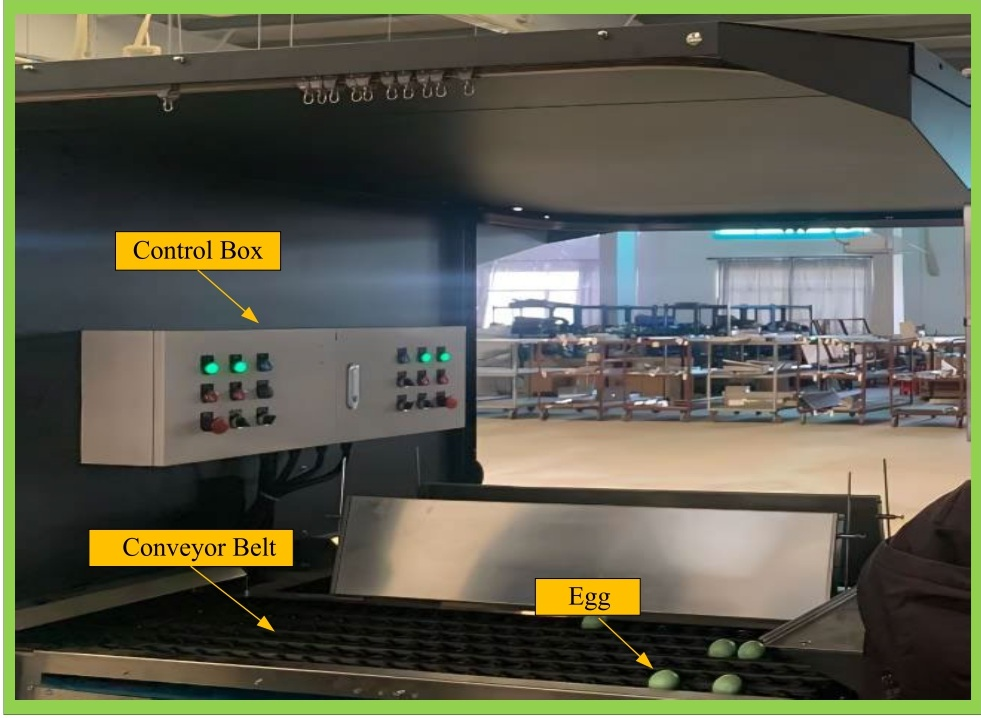
\includegraphics[width=0.65\textwidth]{figure1_egg_conveying_device.jpg}
    \caption{Structural schematic and operational overview of the egg conveying device}
    \label{fig:conveyor_device}
\end{figure}

The conveying mechanism consists of drive chains, transmission gears, bearing blocks and grooved rotating rollers. As eggs transition from the feeding hopper onto the conveyor, each egg rests between two adjacent contoured rollers. The conveyor mechanism imparts dual kinematic motion: forward translational motion along the conveyor line and continuous axial rotation around each egg's major axis. By the time an egg traverses the optical imaging zone, it completes at least one full 360-degree rotation, presenting its entire circumferential shell surface to the overhead machine vision camera and eliminating geometric occlusion blind spots.

\section{Machine Vision Image Acquisition Setup}

The optical acquisition rig is integrated directly above the six-channel conveyor bed within a light-isolated inspection hood. Figure~\ref{fig:vision_system} displays the complete machine vision image acquisition architecture.

\begin{figure}[H]
    \centering
    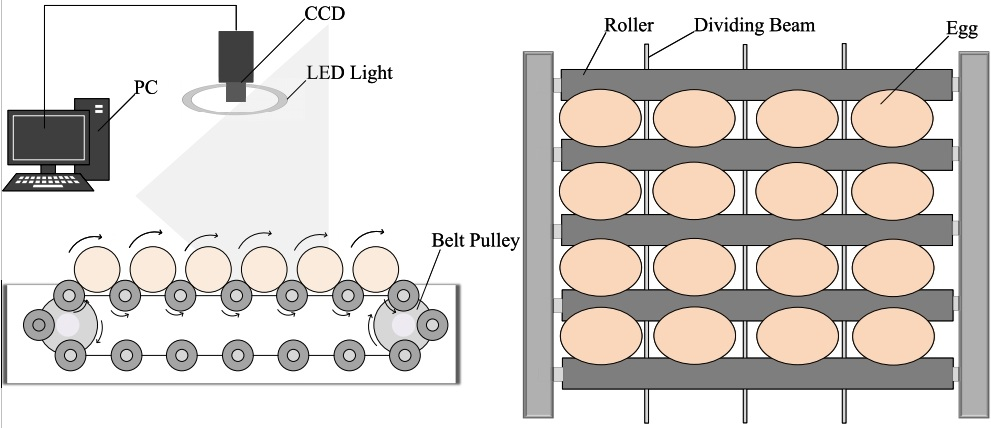
\includegraphics[width=0.92\textwidth]{figure2_machine_vision_system.jpg}
    \caption{Machine vision system architecture and industrial camera installation}
    \label{fig:vision_system}
\end{figure}

The vision system comprises an industrial charge-coupled device (CCD) area-scan camera paired with a low-distortion fixed-focal-length optical lens. Illumination is provided by a high-uniformity diffuse white LED planar light box positioned above the rollers. The LED array operates with high-frequency pulse-width modulation to eliminate camera rolling-shutter flicker. The optical axis of the camera is aligned perpendicular to the conveyor plane, capturing high-resolution planar color frames ($640 \times 640$ pixels) covering all six lanes simultaneously.

\section{Image Dataset Acquisition and Augmentation}

The image dataset was collected on a live industrial egg processing line at Guangzhou Suiping Enterprise Co., Ltd. Unlike laboratory datasets composed of pre-washed, sanitized eggs, the eggs utilized in this study were collected directly from laying hen facilities without preliminary washing. Consequently, the eggshells naturally carried varying amounts of surface contaminants, including fine dust particles, feather fragments and dried manure streaks, reflecting genuine commercial conditions.

Dynamic video sequences of rolling eggs were recorded under production conditions and sliced into discrete frames at regular intervals. Shell cracks were annotated using LabelMe by poultry inspection experts under three distinct target classes. The dataset contains 3,222 high-resolution images, partitioned into training, validation and testing subsets in an approximate ratio of 92:4:4. Table~\ref{tab:dataset_distribution} details the composition of the dataset.

\begin{table}[H]
\centering
\caption{Dataset composition across partitions and defect categories}
\label{tab:dataset_distribution}
\vspace{0.2cm}
\setlength{\tabcolsep}{6pt}
\renewcommand{\arraystretch}{1.15}
\small
\begin{tabular}{|l|c|c|c|c|}
\hline
\textbf{Partition} & \textbf{Images} & \textbf{Intact Eggs (Cat 1)} & \textbf{Cracked Eggs (Cat 2)} & \textbf{Crack Regions (Cat 3)} \\
\hline
Training Set & 2,972 & 7,015 & 2,501 & 2,708 \\
Validation Set & 126 & 298 & 105 & 114 \\
Test Set & 125 & 298 & 105 & 113 \\
\hline
\textbf{Total} & \textbf{3,222} & \textbf{7,611} & \textbf{2,711} & \textbf{2,935} \\
\hline
\end{tabular}
\end{table}

Data augmentation strategies, including random horizontal flips, mosaic synthesis, HSV color space jittering and random affine transformations, were applied during offline training to expand sample diversity and prevent overfitting.

\section{Triple Classification Granularity Paradigm}

Conventional agricultural defect inspection frameworks formulate egg grading as a binary classification problem: classifying each candidate region simply as intact or cracked. However, binary classification exhibits inherent vulnerabilities in dynamic factory environments. A small hairline crack on an unwashed shell may produce subtle feature activation that falls below the global decision threshold, leading to a missed detection.

To address this limitation, the proposed method establishes a triple classification granularity framework, illustrated in Figure~\ref{fig:categories}:
\begin{itemize}
    \item \textbf{Category 1 (Intact Egg):} The entire egg body exhibiting a continuous, structurally unbroken shell without fractures or punctures.
    \item \textbf{Category 2 (Cracked Egg):} The entire egg body containing one or more visible shell cracks, representing an egg-level macro-defect label.
    \item \textbf{Category 3 (Crack Region):} A tight bounding box tightly circumscribing the localized fracture zone, micro-crack line or puncture epicenter, representing a micro-level defect label.
\end{itemize}

\begin{figure}[H]
    \centering
    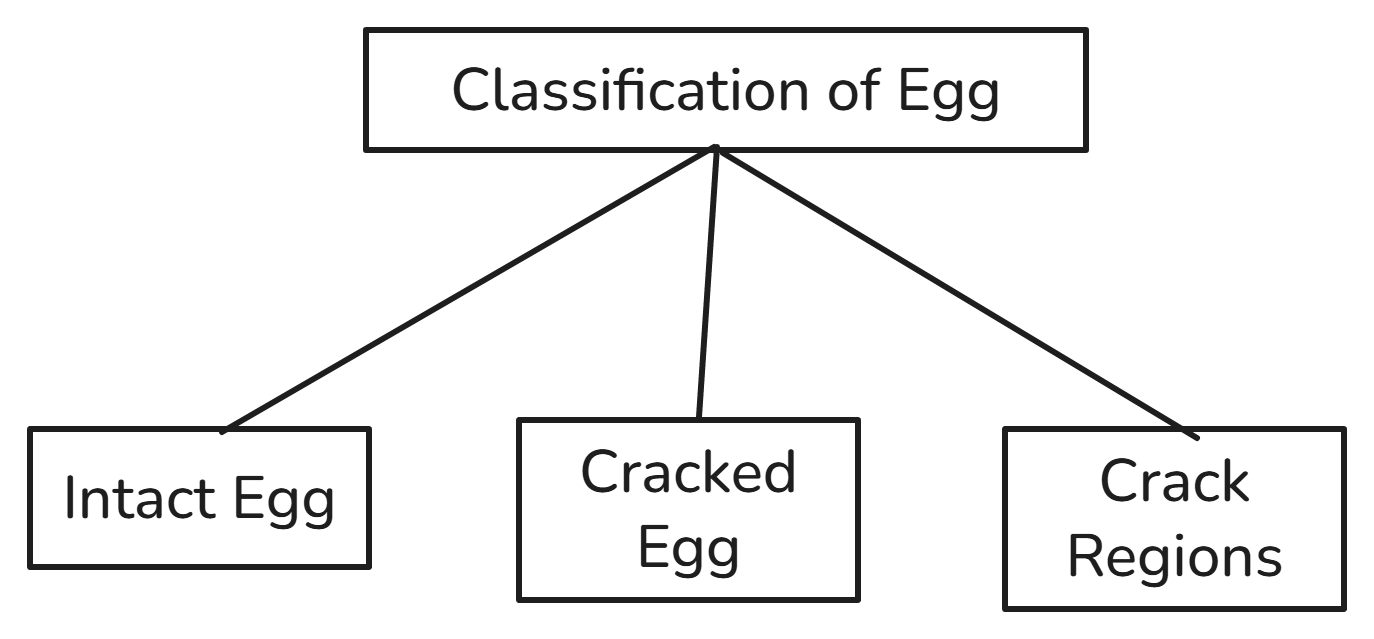
\includegraphics[width=0.78\textwidth]{classificationCategories.png}
    \caption{Triple classification granularity scheme: Intact Egg, Cracked Egg and Crack Region}
    \label{fig:categories}
\end{figure}

This multi-granularity formulation provides simultaneous multi-scale supervision during backpropagation. The network learns both holistic egg body representations and high-frequency local crack edge patterns, establishing redundant feature pathways.

\section{Baseline YOLOv8 Architecture and Detected Limitations}

YOLOv8 represents a cutting-edge, single-stage object detector known for high speed and accuracy. It features a CSPDarknet backbone with C2f (Cross Stage Partial with two convolutions) modules, an SPPF (Spatial Pyramid Pooling Fast) block and an anchor-free decoupled detection head that independently predicts bounding box coordinates and class probability distributions.

Despite its general-purpose effectiveness, standard YOLOv8 suffers from structural shortcomings when applied to hairline crack inspection on unwashed eggs:
\begin{enumerate}[label=\arabic*.]
    \item \textbf{Rigid Convolutional Sampling:} Standard $3 \times 3$ convolutional kernels operate over fixed rectangular grids. Hairline cracks follow jagged, tortuous trajectories, causing rigid kernels to sample irrelevant background shell texture and diluting crack gradients.
    \item \textbf{Loss of Micro-Crack Information:} Standard YOLOv8 downsamples inputs by $32\times$, producing detection heads at P3 ($80 \times 80$), P4 ($40 \times 40$) and P5 ($20 \times 20$). Minute hairline cracks occupying widths under 0.1 mm vanish across successive pooling layers.
    \item \textbf{Static IoU Loss Weighting:} The default CIoU loss applies static geometric penalties that over-penalize extreme low-quality outlier bounding boxes while insufficiently penalizing hard, medium-quality crack candidates.
\end{enumerate}

\section{Proposed Improved YOLOv8 Network Architecture}

To overcome these structural limitations, four key enhancements were integrated into the YOLOv8 architecture: embedding Deformable Convolution v2 (DCNv2) into the backbone, incorporating a Weighted Bidirectional Feature Pyramid Network (BiFPN), adding a dedicated P2 small target detection head and adopting Wise-IoU v2 (WIoUv2) loss.

Figure~\ref{fig:yolov8_arch} displays the complete architectural layout of the proposed improved YOLOv8 network.

\begin{figure}[H]
    \centering
    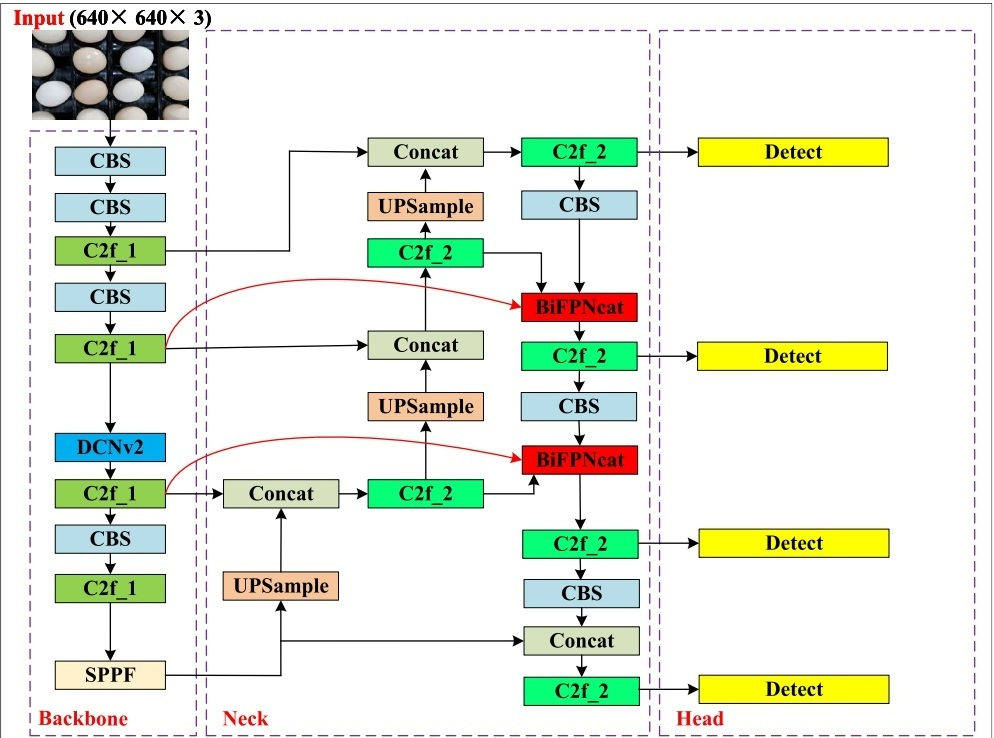
\includegraphics[width=0.90\textwidth]{figure3_improved_yolov8_architecture_1.jpg}
    \caption{Detailed architectural layout of the improved YOLOv8 framework}
    \label{fig:yolov8_arch}
\end{figure}

The network processes $640 \times 640$ RGB frames. The backbone extracts feature maps at progressive strides, passing enriched feature hierarchies to the multi-scale BiFPN neck and four decoupled detection heads (P2, P3, P4, P5).

\section{Deformable Convolution v2 (DCNv2) Module}

Standard 2D convolution evaluates feature maps across a rigid rectangular grid $\mathcal{R}$. For a $3 \times 3$ kernel, the regular sampling grid is defined as:
\begin{equation}
\mathcal{R} = \{(-1,-1), (-1,0), (-1,1), (0,-1), (0,0), (0,1), (1,-1), (1,0), (1,1)\}
\end{equation}
The output feature vector $Y$ at spatial location $p_0$ is computed as:
\begin{equation}
Y(p_0) = \sum_{p_n \in \mathcal{R}} w(p_n) \cdot X(p_0 + p_n)
\end{equation}
where $X$ is the input feature map and $w(p_n)$ represents kernel weight parameters.

Because crack paths follow winding, irregular biological contours, rigid sampling points often fall onto intact shell surfaces or adjacent dirt particles. Deformable Convolution v2 (DCNv2) introduces learnable 2D spatial coordinate offsets $\Delta p_n$ and modulation scalar values $\Delta m_n \in [0, 1]$:
\begin{equation}
Y(p_0) = \sum_{p_n \in \mathcal{R}} w(p_n) \cdot X(p_0 + p_n + \Delta p_n) \cdot \Delta m_n
\end{equation}
where $\Delta p_n$ allows the sampling grid to freely deform along the curvilinear contour of the crack and $\Delta m_n$ modulates feature amplitude, suppressing non-crack shell textures.

Figure~\ref{fig:dcnv2_sampling} compares standard rectangular convolution sampling grids with deformable sampling point distributions along irregular crack fissures.

\begin{figure}[H]
    \centering
    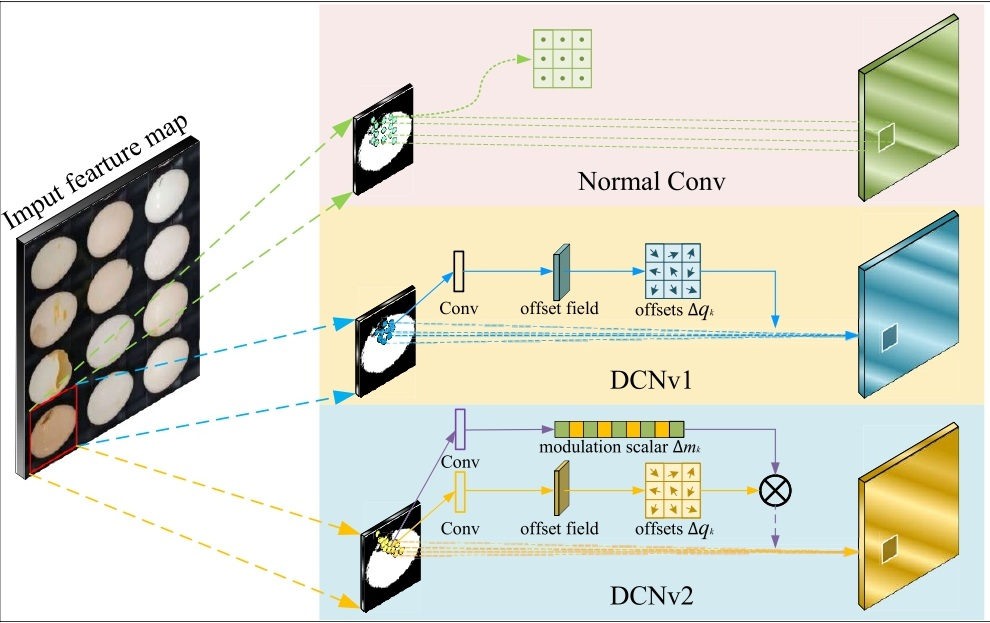
\includegraphics[width=0.75\textwidth]{figure4_dcnv2_sampling_comparison.jpg}
    \caption{Comparison of regular convolution sampling and DCNv2 deformable sampling on irregular cracks}
    \label{fig:dcnv2_sampling}
\end{figure}

The offsets $\Delta p_n$ and modulation scalars $\Delta m_n$ are generated by applying a lightweight parallel convolution layer over the input features, enabling end-to-end differentiable training.

\section{Weighted BiFPN Neck and P2 Small Target Detection Head}

In the baseline YOLOv8, feature fusion is handled by the PANet architecture, which aggregates multi-scale features through sequential top-down and bottom-up pathways using uniform unweighted addition. However, features from different pyramid levels contribute unequally to defect detection: shallow layers carry high-resolution spatial details essential for micro-cracks, while deep layers carry rich semantic context.

The Weighted Bidirectional Feature Pyramid Network (BiFPN) optimizes multi-scale fusion through three key mechanisms:
\begin{enumerate}[label=\arabic*.]
    \item \textbf{Node Pruning:} Nodes with only a single input edge are eliminated, as they contribute minimal feature transformation while adding computational cost.
    \item \textbf{Cross-Scale Residual Connections:} Direct residual connections are added between original input nodes and output nodes at the same scale, preserving shallow spatial cues.
    \item \textbf{Fast Normalized Feature Fusion:} Features are merged using learnable normalized weights:
    \begin{equation}
    O = \sum_{i} \frac{w_i}{\epsilon + \sum_{j} w_j} \cdot I_i
    \end{equation}
    where $w_i \ge 0$ is a learnable scalar weight enforced via ReLU activation, $I_i$ is the feature map at pathway $i$ and $\epsilon = 0.0001$ prevents numerical instability.
\end{enumerate}

Figure~\ref{fig:bifpn_structure} compares the architectural topologies of FPN, PANet and the Weighted BiFPN.

\begin{figure}[H]
    \centering
    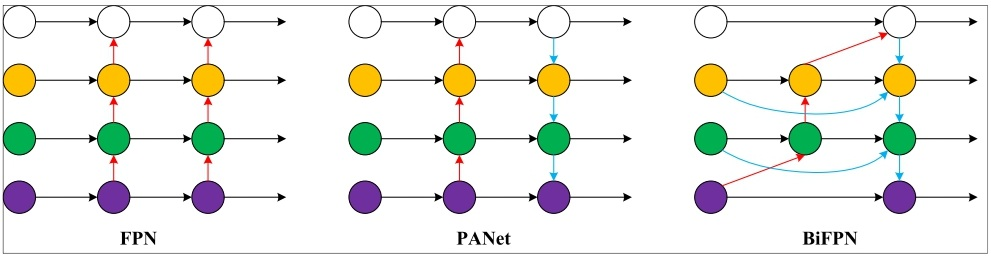
\includegraphics[width=0.95\textwidth]{figure5_fpn_panet_bifpn_structure.jpg}
    \caption{Architectural comparison of multi-scale feature fusion structures: FPN, PANet and BiFPN}
    \label{fig:bifpn_structure}
\end{figure}

To further preserve micro-crack details, a dedicated P2 small target detection head is added to the network. Operating on a $160 \times 160$ feature map (stride 4, $4 \times 4$ pixel receptive field), this head captures sub-millimeter fissure boundaries that would otherwise be obliterated by the stride-32 downsampling of standard YOLOv8.

\section{Wise-IoU v2 Dynamic Bounding Box Loss Formulation}

Bounding box regression accuracy directly determines crack localization precision. The conventional CIoU loss used in YOLOv8 considers bounding box overlap, center point distance and aspect ratio consistency. However, CIoU enforces static geometric penalties that disproportionately penalize low-quality outlier bounding boxes caused by ambiguous crack shadows or surface dirt.

Wise-IoU v2 (WIoUv2) introduces a dynamic non-monotonic focusing mechanism based on an outlier degree metric $\beta$:
\begin{equation}
\beta = \frac{L_{\text{IoU}}}{\overline{L_{\text{IoU}}}} \in [0, +\infty)
\end{equation}
where $L_{\text{IoU}} = 1 - \text{IoU}$ and $\overline{L_{\text{IoU}}}$ is the running exponential moving average of the IoU loss across batches.

The outlier degree $\beta$ quantifies sample difficulty: a small $\beta$ indicates an easy, high-quality anchor, while a large $\beta$ indicates a severe low-quality outlier. WIoUv2 constructs a dynamic non-monotonic focusing coefficient $r$:
\begin{equation}
r = \frac{\beta}{\delta \alpha^{\beta - \delta}}
\end{equation}
where $\alpha$ and $\delta$ are hyperparameter constants governing gradient distribution.

The total WIoUv2 bounding box loss is formulated as:
\begin{equation}
L_{\text{WIoUv2}} = r \cdot L_{\text{WIoUv1}} = r \cdot \mathcal{R}_{\text{WIoU}} \cdot L_{\text{IoU}}
\end{equation}
where $\mathcal{R}_{\text{WIoU}} \in [1, e)$ is the distance penalty term:
\begin{equation}
\mathcal{R}_{\text{WIoU}} = \exp\left( \frac{(x - x_{gt})^2 + (y - y_{gt})^2}{(W_g)^2 + (H_g)^2} \right)
\end{equation}
Here, $(x, y)$ and $(x_{gt}, y_{gt})$ denote predicted and ground-truth bounding box center coordinates and $W_g, H_g$ represent the width and height of the smallest enclosing bounding box. By assigning smaller gradient weights to extreme outliers and prioritizing moderately challenging candidates, WIoUv2 achieves superior bounding box alignment on irregular hairline cracks.

\section{Dual Verification Mechanism and Redundant Decision Logic}

In high-speed commercial sorting lines, false negatives (escaped cracked eggs) cause batch-wide bacterial contamination, while false positives (discarded intact eggs) inflict direct financial losses. To achieve near-zero escape rates without excessive false alarms, the framework introduces a redundant dual verification decision mechanism operating on the triple granularity outputs.

Let $D_1, D_2, D_3$ denote the binary detection outcomes for Category 1 (Intact Egg), Category 2 (Cracked Egg) and Category 3 (Crack Region) respectively within the spatial bounding volume of an individual egg pocket. The final sorting decision is governed by two complementary rules:
\begin{enumerate}[label=\arabic*.]
    \item \textbf{Cracked Egg Classification Rule (Union Logic):} An egg is classified as cracked if either the holistic cracked egg detector fires or the localized crack region detector fires:
    \begin{equation}
    \text{Status} = \text{Cracked} \iff (D_2 = 1) \lor (D_3 = 1)
    \end{equation}
    \item \textbf{Intact Egg Classification Rule (Intersection Logic):} An egg is classified as intact if and only if Category 1 is positively identified and neither Category 2 nor Category 3 is detected:
    \begin{equation}
    \text{Status} = \text{Intact} \iff (D_1 = 1) \land (D_2 = 0) \land (D_3 = 0)
    \end{equation}
\end{enumerate}

Assuming the error probabilities of the macro-scale detector ($P(\text{Miss}_{\text{Cat2}})$) and micro-scale detector ($P(\text{Miss}_{\text{Cat3}})$) are statistically independent, the compound miss probability under dual verification is:
\begin{equation}
P(\text{Miss}_{\text{Compound}}) = P(\text{Miss}_{\text{Cat2}}) \times P(\text{Miss}_{\text{Cat3}})
\end{equation}
Because both individual miss rates are fractional values, their mathematical product reduces defect escape rates by an order of magnitude.

\section{Offline Model Training and Online Inference Framework}

The end-to-end technical pipeline bridges offline deep model training with high-speed online conveyor sorting. Figure~\ref{fig:training_schematic} illustrates the offline training and online deployment workflow.

\begin{figure}[H]
    \centering
    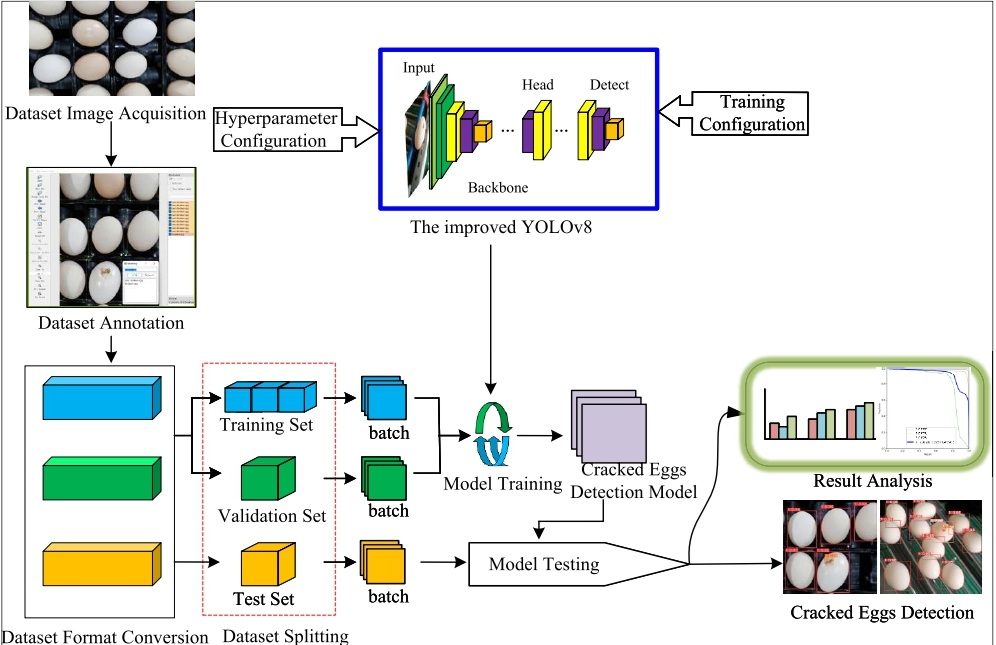
\includegraphics[width=0.95\textwidth]{figure6_training_schematic.jpg}
    \caption{Comprehensive technical workflow spanning offline training, model export and online inference}
    \label{fig:training_schematic}
\end{figure}

During offline training, unwashed egg images are augmented and fed into the improved YOLOv8 model for 300 epochs. Gradients are computed via backpropagation across the multi-task loss function combining WIoUv2 bounding box regression and BCE classification loss. The trained model weights are exported and optimized for inference using TensorRT.

During online operation, the industrial camera captures live conveyor frames at 45 FPS. The Python inference engine executes bounding box prediction, applies non-maximum suppression (NMS) and evaluates dual verification logic to transmit sorting commands to downstream pneumatic sorting actuators.

\section{Experimental Setup and Hyperparameter Configuration}

The computational environment and hyperparameters utilized for offline model training and comparative evaluation are summarized in Table~\ref{tab:hardware_software}.

\begin{table}[H]
\centering
\caption{Computational hardware specifications and software environment}
\label{tab:hardware_software}
\vspace{0.2cm}
\setlength{\tabcolsep}{8pt}
\renewcommand{\arraystretch}{1.15}
\small
\begin{tabular}{|l|l|}
\hline
\textbf{Component / Parameter} & \textbf{Specification / Value} \\
\hline
Operating System & Microsoft Windows 10 (64-bit) \\
\hline
Central Processing Unit (CPU) & Intel Core i5-10400F @ 2.90 GHz \\
\hline
Graphics Processing Unit (GPU) & NVIDIA GeForce RTX 3060 (12 GB VRAM) \\
\hline
System Memory (RAM) & 32 GB DDR4 (3200 MHz) \\
\hline
Framework and Language & PyTorch 1.13.1, CUDA 11.6, Python 3.8 \\
\hline
Image Resolution & $640 \times 640$ pixels \\
\hline
Training Epochs and Batch Size & 300 epochs, batch size 16 \\
\hline
Optimizer and Initial LR & SGD (momentum: 0.937), initial lr: 0.01 \\
\hline
\end{tabular}
\end{table}

\section{Quantitative Evaluation Metrics}

Model detection performance is quantitatively evaluated using standard computer vision metrics: Precision, Recall, Mean Average Precision at IoU threshold 0.5 (mAP@0.5), False Negative Rate (FNR), False Positive Rate (FPR) and Frames Per Second (FPS):
\begin{equation}
\text{Precision} = \frac{\text{TP}}{\text{TP} + \text{FP}}, \quad \text{Recall} = \frac{\text{TP}}{\text{TP} + \text{FN}}
\end{equation}
\begin{equation}
\text{mAP@0.5} = \frac{1}{N_c} \sum_{i=1}^{N_c} \text{AP}_i, \quad \text{FNR} = \frac{\text{FN}}{\text{TP} + \text{FN}}, \quad \text{FPR} = \frac{\text{FP}}{\text{FP} + \text{TN}}
\end{equation}
where TP, FP, TN and FN denote true positives, false positives, true negatives and false negatives respectively, $N_c = 3$ is the number of target categories and $\text{AP}_i$ represents the area under the Precision-Recall curve for category $i$.

%=========================================================
% CHAPTER 3: RESULTS AND ANALYSIS
%=========================================================

\chapter{Results and Analysis}

\section{Ablation Study: Impact of Proposed Structural Components}

To quantify the individual and synergistic contributions of DCNv2, BiFPN, WIoUv2 and the P2 small target detection head, eight systematic ablation experiments were conducted on the unwashed egg test dataset under identical training protocols. Table~\ref{tab:ablation_results} presents the ablation results across all eight model configurations.

\begin{table}[H]
\centering
\caption{Ablation experiment results on test dataset}
\label{tab:ablation_results}
\vspace{0.2cm}
\setlength{\tabcolsep}{6pt}
\renewcommand{\arraystretch}{1.15}
\small
\begin{tabular}{|c|c|c|c|c|c|c|}
\hline
\textbf{DCNv2} & \textbf{BiFPN} & \textbf{WIoU} & \textbf{Small Target Head} & \textbf{Precision (\%)} & \textbf{Recall (\%)} & \textbf{mAP@0.5 (\%)} \\
\hline
- & - & - & - & 92.2 & 85.3 & 87.7 \\
\hline
- & - & \checkmark & - & 90.6 & 87.4 & 90.3 \\
\hline
- & \checkmark & - & - & 89.8 & 83.8 & 88.2 \\
\hline
- & - & - & \checkmark & 93.8 & 90.3 & 93.0 \\
\hline
\checkmark & - & \checkmark & - & 93.1 & 89.4 & 92.1 \\
\hline
- & \checkmark & \checkmark & - & 92.6 & 89.5 & 92.2 \\
\hline
\checkmark & \checkmark & \checkmark & - & 93.8 & 89.9 & 92.6 \\
\hline
\checkmark & \checkmark & \checkmark & \checkmark & \textbf{94.1} & \textbf{90.0} & \textbf{92.9} \\
\hline
\end{tabular}
\end{table}

Key analytical findings from the ablation evaluations:
\begin{enumerate}[label=\arabic*.]
    \item \textbf{Impact of WIoUv2 Dynamic Loss:} Replacing the default CIoU loss with WIoUv2 increased mAP@0.5 from 87.7\% to 90.3\% (+2.6 percentage points), demonstrating that dynamic gradient allocation effectively reduces the disruptive influence of extreme low-quality bounding box outliers.
    \item \textbf{Impact of P2 Small Target Detection Head:} Introducing the P2 detection head yielded the single largest performance gain (+5.3\% mAP@0.5), boosting recall from 85.3\% to 90.3\%. Operating on high-resolution $160 \times 160$ feature maps preserves the faint edge gradients of micro-cracks that are lost in standard stride-32 downsampling.
    \item \textbf{Synergy of DCNv2 and BiFPN:} Adding DCNv2 and BiFPN alongside WIoUv2 and the P2 head produced the most balanced overall performance, achieving 94.1\% precision, 90.0\% recall and 92.9\% mAP@0.5 (+5.2\% improvement over baseline YOLOv8). DCNv2 dynamically conforms receptive fields to winding crack trajectories, while BiFPN ensures robust cross-scale feature fusion across varying lighting angles.
\end{enumerate}

\section{Model Complexity and Computational Overhead Analysis}

Table~\ref{tab:model_complexity} presents a comparative analysis of model complexity and computational footprint between baseline YOLOv8 and the proposed improved YOLOv8 framework.

\begin{table}[H]
\centering
\caption{Model complexity and computational footprint comparison}
\label{tab:model_complexity}
\vspace{0.2cm}
\setlength{\tabcolsep}{10pt}
\renewcommand{\arraystretch}{1.15}
\small
\begin{tabular}{|l|c|c|c|}
\hline
\textbf{Model Architecture} & \textbf{Parameters} & \textbf{FLOPs (G)} & \textbf{Model Size (MB)} \\
\hline
Baseline YOLOv8 & $2.59 \times 10^7$ & 79.1 & 49.6 \\
\hline
Proposed Improved YOLOv8 & $2.66 \times 10^7$ & 86.5 & 51.1 \\
\hline
\textbf{Relative Increase} & \textbf{+2.7\%} & \textbf{+9.3\%} & \textbf{+3.0\%} \\
\hline
\end{tabular}
\end{table}

The structural enhancements introduce minimal computational overhead: model parameters increase by only 2.7\% (from $2.59 \times 10^7$ to $2.66 \times 10^7$), floating-point operations increase by 9.3\% (from 79.1 G to 86.5 G FLOPs) and disk storage footprint increases by just 1.5 MB (from 49.6 MB to 51.1 MB). This modest complexity overhead makes the model well-suited for industrial edge deployment.

\section{Comparative Performance Benchmark Against Mainstream Detectors}

To establish comparative superiority, the proposed model was benchmarked against leading two-stage and single-stage object detectors on the identical unwashed egg test dataset. Table~\ref{tab:benchmark_comparison} summarizes performance metrics across all evaluated architectures.

\begin{table}[H]
\centering
\caption{Comparative performance benchmark across mainstream detectors}
\label{tab:benchmark_comparison}
\vspace{0.2cm}
\setlength{\tabcolsep}{8pt}
\renewcommand{\arraystretch}{1.15}
\small
\begin{tabular}{|l|c|c|c|c|}
\hline
\textbf{Object Detection Model} & \textbf{Precision (\%)} & \textbf{Recall (\%)} & \textbf{mAP@0.5 (\%)} & \textbf{Speed (FPS)} \\
\hline
Faster R-CNN (ResNet50) & 68.4 & 80.7 & 78.1 & 17 \\
\hline
YOLOv5 & 86.9 & 81.1 & 85.2 & 58 \\
\hline
YOLOv8 (Baseline) & 92.2 & 85.3 & 87.7 & 52 \\
\hline
YOLOv11 & 92.7 & 84.3 & 87.3 & 47 \\
\hline
\textbf{Proposed Improved YOLOv8} & \textbf{94.1} & \textbf{90.0} & \textbf{92.9} & \textbf{45} \\
\hline
\end{tabular}
\end{table}

The proposed model outperforms all competing architectures across precision, recall and mAP@0.5:
\begin{itemize}
    \item Faster R-CNN achieves only 78.1\% mAP@0.5 and operates at 17 FPS, failing industrial speed thresholds ($\ge 30$ FPS).
    \item YOLOv5 achieves 85.2\% mAP@0.5, suffering from missed detections on fine hairline fissures.
    \item YOLOv11 achieves 87.3\% mAP@0.5, performing comparably to baseline YOLOv8 (87.7\%) but lacking specialized receptive field adaptation.
    \item The proposed model achieves 92.9\% mAP@0.5, outperforming baseline YOLOv8 by +5.2 percentage points and Faster R-CNN by +14.8 percentage points while operating at 45 FPS, comfortably exceeding the 30 FPS real-time conveyor sorting requirement.
\end{itemize}

\section{Precision-Recall Dynamics and Defect-Specific Performance}

Figure~\ref{fig:pr_curves} displays the Precision-Recall (PR) curves for baseline YOLOv8 and the proposed improved YOLOv8 across all three defect categories.

\begin{figure}[H]
    \centering
    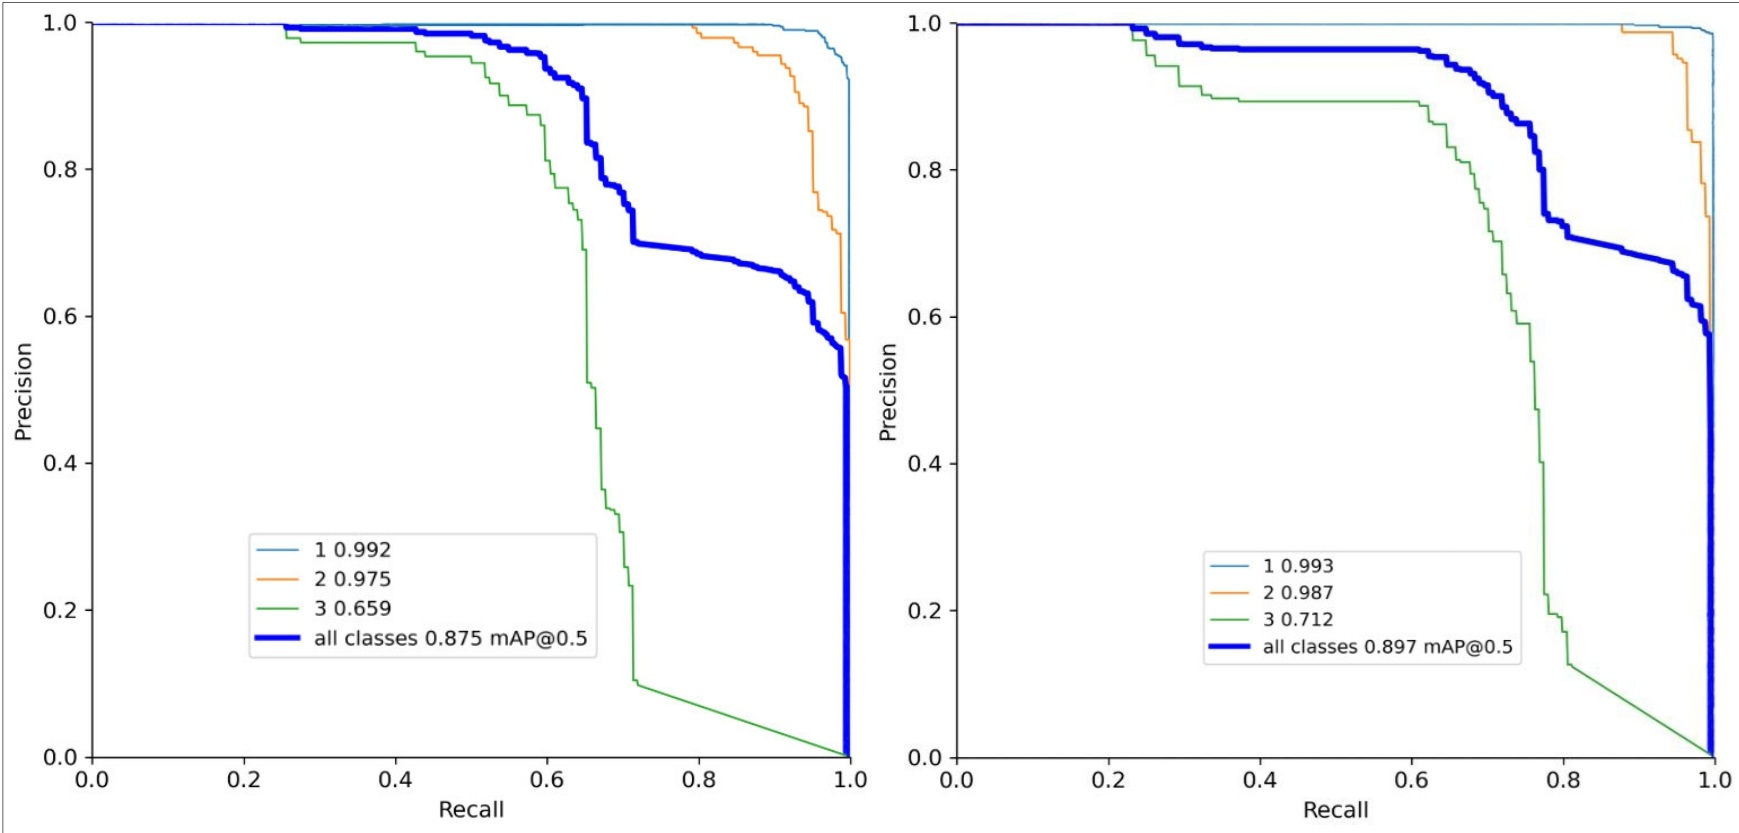
\includegraphics[width=0.95\textwidth]{figure8_pr_curves_comparison.jpg}
    \caption{Precision-Recall curves comparison between baseline YOLOv8 and the proposed model across all target categories}
    \label{fig:pr_curves}
\end{figure}

The area under the PR curve expands substantially for the proposed model across all categories. The most pronounced expansion occurs in Category 3 (Crack Region), where the addition of the P2 small target head and DCNv2 enables sustained high precision even at high recall operating points.

\section{Visual Detection Performance and Comparison}

Figure~\ref{fig:visual_detection} provides visual detection comparisons between Faster R-CNN, YOLOv5, baseline YOLOv8 and the proposed improved model under challenging factory conditions.

\begin{figure}[H]
    \centering
    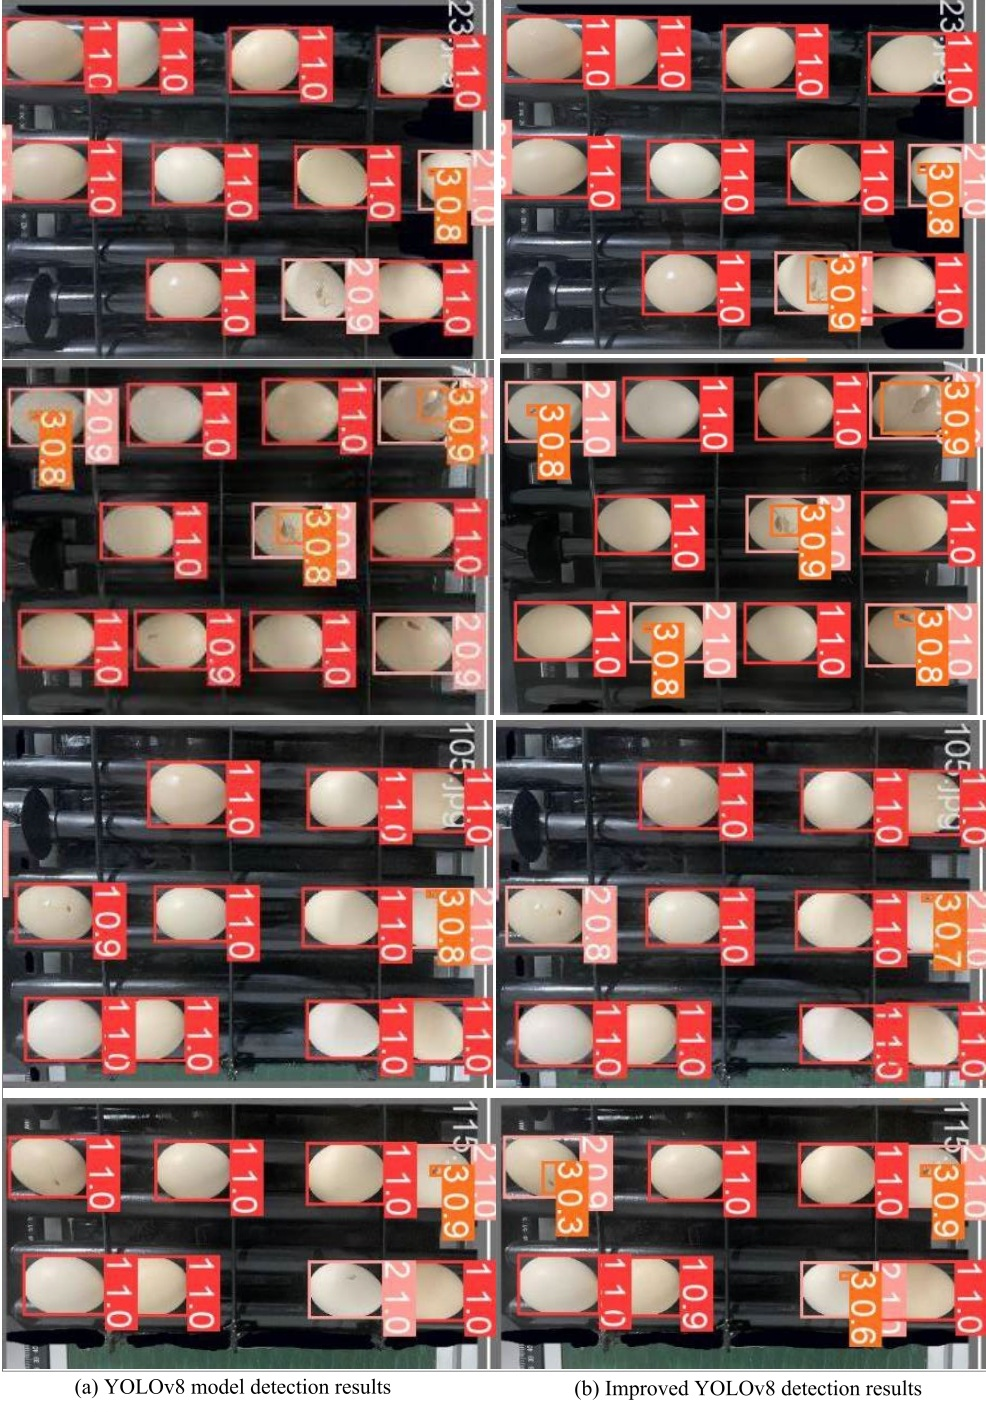
\includegraphics[width=0.80\textwidth]{figure9_detection_effects_comparison.jpg}
    \caption{Visual detection comparisons of Faster R-CNN, YOLOv5, baseline YOLOv8 and the proposed improved model on unwashed eggs}
    \label{fig:visual_detection}
\end{figure}

In challenging scenarios featuring unwashed eggs with surface manure streaks and faint micro-cracks, Faster R-CNN and YOLOv5 frequently produce false positive detections on surface stains. Baseline YOLOv8 misses low-contrast hairline fissures. In contrast, the proposed improved YOLOv8 accurately identifies the holistic cracked egg boundary while tightly segmenting localized crack regions without being misled by non-defective surface contaminants.

\section{Industrial Conveyor Online Dynamic Testing}

To validate real-world operational efficacy, the trained model was deployed onto an active industrial egg conveyor grading system at Guangzhou Suiping Enterprise Co., Ltd. Figure~\ref{fig:online_deployment} illustrates the online production testing environment.

\begin{figure}[H]
    \centering
    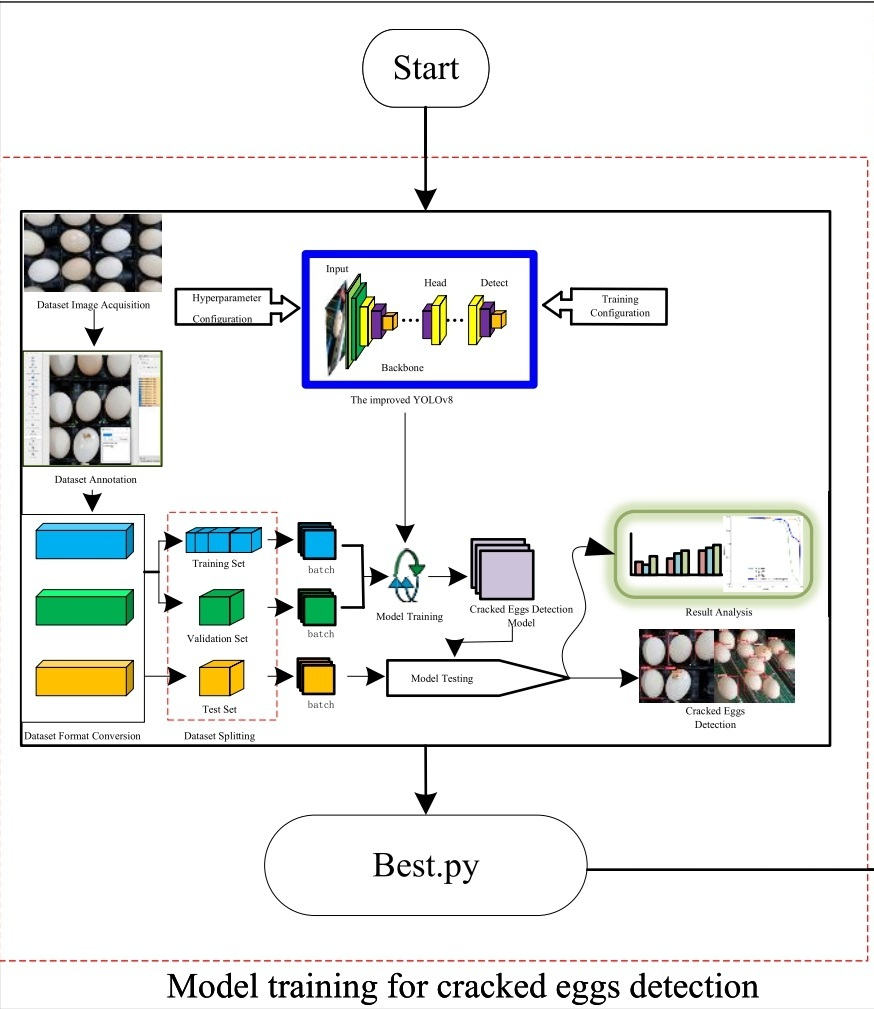
\includegraphics[width=0.75\textwidth]{figure7_online_deployment_testing_1.jpg}
    \caption{Online deployment and testing on the industrial egg conveyor line}
    \label{fig:online_deployment}
\end{figure}

The online testing system operates across six parallel channels. Eggs translate forward while rotating axially over contoured rollers. An industrial camera records continuous video streams at 45 FPS and each individual egg is tracked across approximately 60 video frames during its passage through the imaging zone.

\section{Online Inspection Accuracy and Dual Verification Validation}

Table~\ref{tab:online_inspection_errors} summarizes online inspection error rates (False Negative Rate and False Positive Rate) evaluated across 106 continuous production video frames.

\begin{table}[H]
\centering
\caption{Online factory inspection error rates across 106 production video frames}
\label{tab:online_inspection_errors}
\vspace{0.2cm}
\setlength{\tabcolsep}{6pt}
\renewcommand{\arraystretch}{1.2}
\small
\begin{tabular}{|l|c|c|c|c|}
\hline
\textbf{Classification Category} & \multicolumn{2}{c|}{\textbf{Baseline YOLOv8}} & \multicolumn{2}{c|}{\textbf{Proposed Improved YOLOv8}} \\
\cline{2-5}
& \textbf{FNR (\%)} & \textbf{FPR (\%)} & \textbf{FNR (\%)} & \textbf{FPR (\%)} \\
\hline
Class 1: Intact Egg & 1.26 & 4.00 & \textbf{0.46} & \textbf{2.18} \\
\hline
Class 2: Cracked Egg & 10.17 & 3.20 & \textbf{5.52} & \textbf{1.16} \\
\hline
Class 3: Damaged Area & 22.97 & 0.87 & \textbf{19.19} & \textbf{0.58} \\
\hline
\textbf{Compound Dual Verification FNR} & \multicolumn{2}{c|}{$10.17\% \times 22.97\% = 2.34\%$} & \multicolumn{2}{c|}{$\mathbf{5.52\% \times 19.19\% = 1.06\%}$} \\
\hline
\end{tabular}
\end{table}

Key findings from industrial online testing:
\begin{enumerate}[label=\arabic*.]
    \item \textbf{Intact Egg False Alarm Reduction:} The false alarm rate (FPR) for intact eggs dropped from 4.00\% to 2.18\%, saving 1.82\% of healthy eggs from erroneous discard.
    \item \textbf{Individual Category Sensitivity:} For cracked eggs (Category 2), the miss rate (FNR) was cut nearly in half from 10.17\% to 5.52\%, while the false positive rate decreased from 3.20\% to 1.16\%.
    \item \textbf{Compound Miss Rate under Dual Verification:} Under dual verification logic, an egg escapes detection only if both Category 2 and Category 3 miss simultaneously. The compound miss rate was driven down to just:
    \begin{equation}
    5.52\% \times 19.19\% = 1.06\%
    \end{equation}
    representing an absolute error reduction of 4.65\% over single-detector setups and satisfying industrial grading criteria.
\end{enumerate}

Figure~\ref{fig:production_detection} displays visual detection outputs on the active multi-channel conveyor bed during online operation.

\begin{figure}[H]
    \centering
    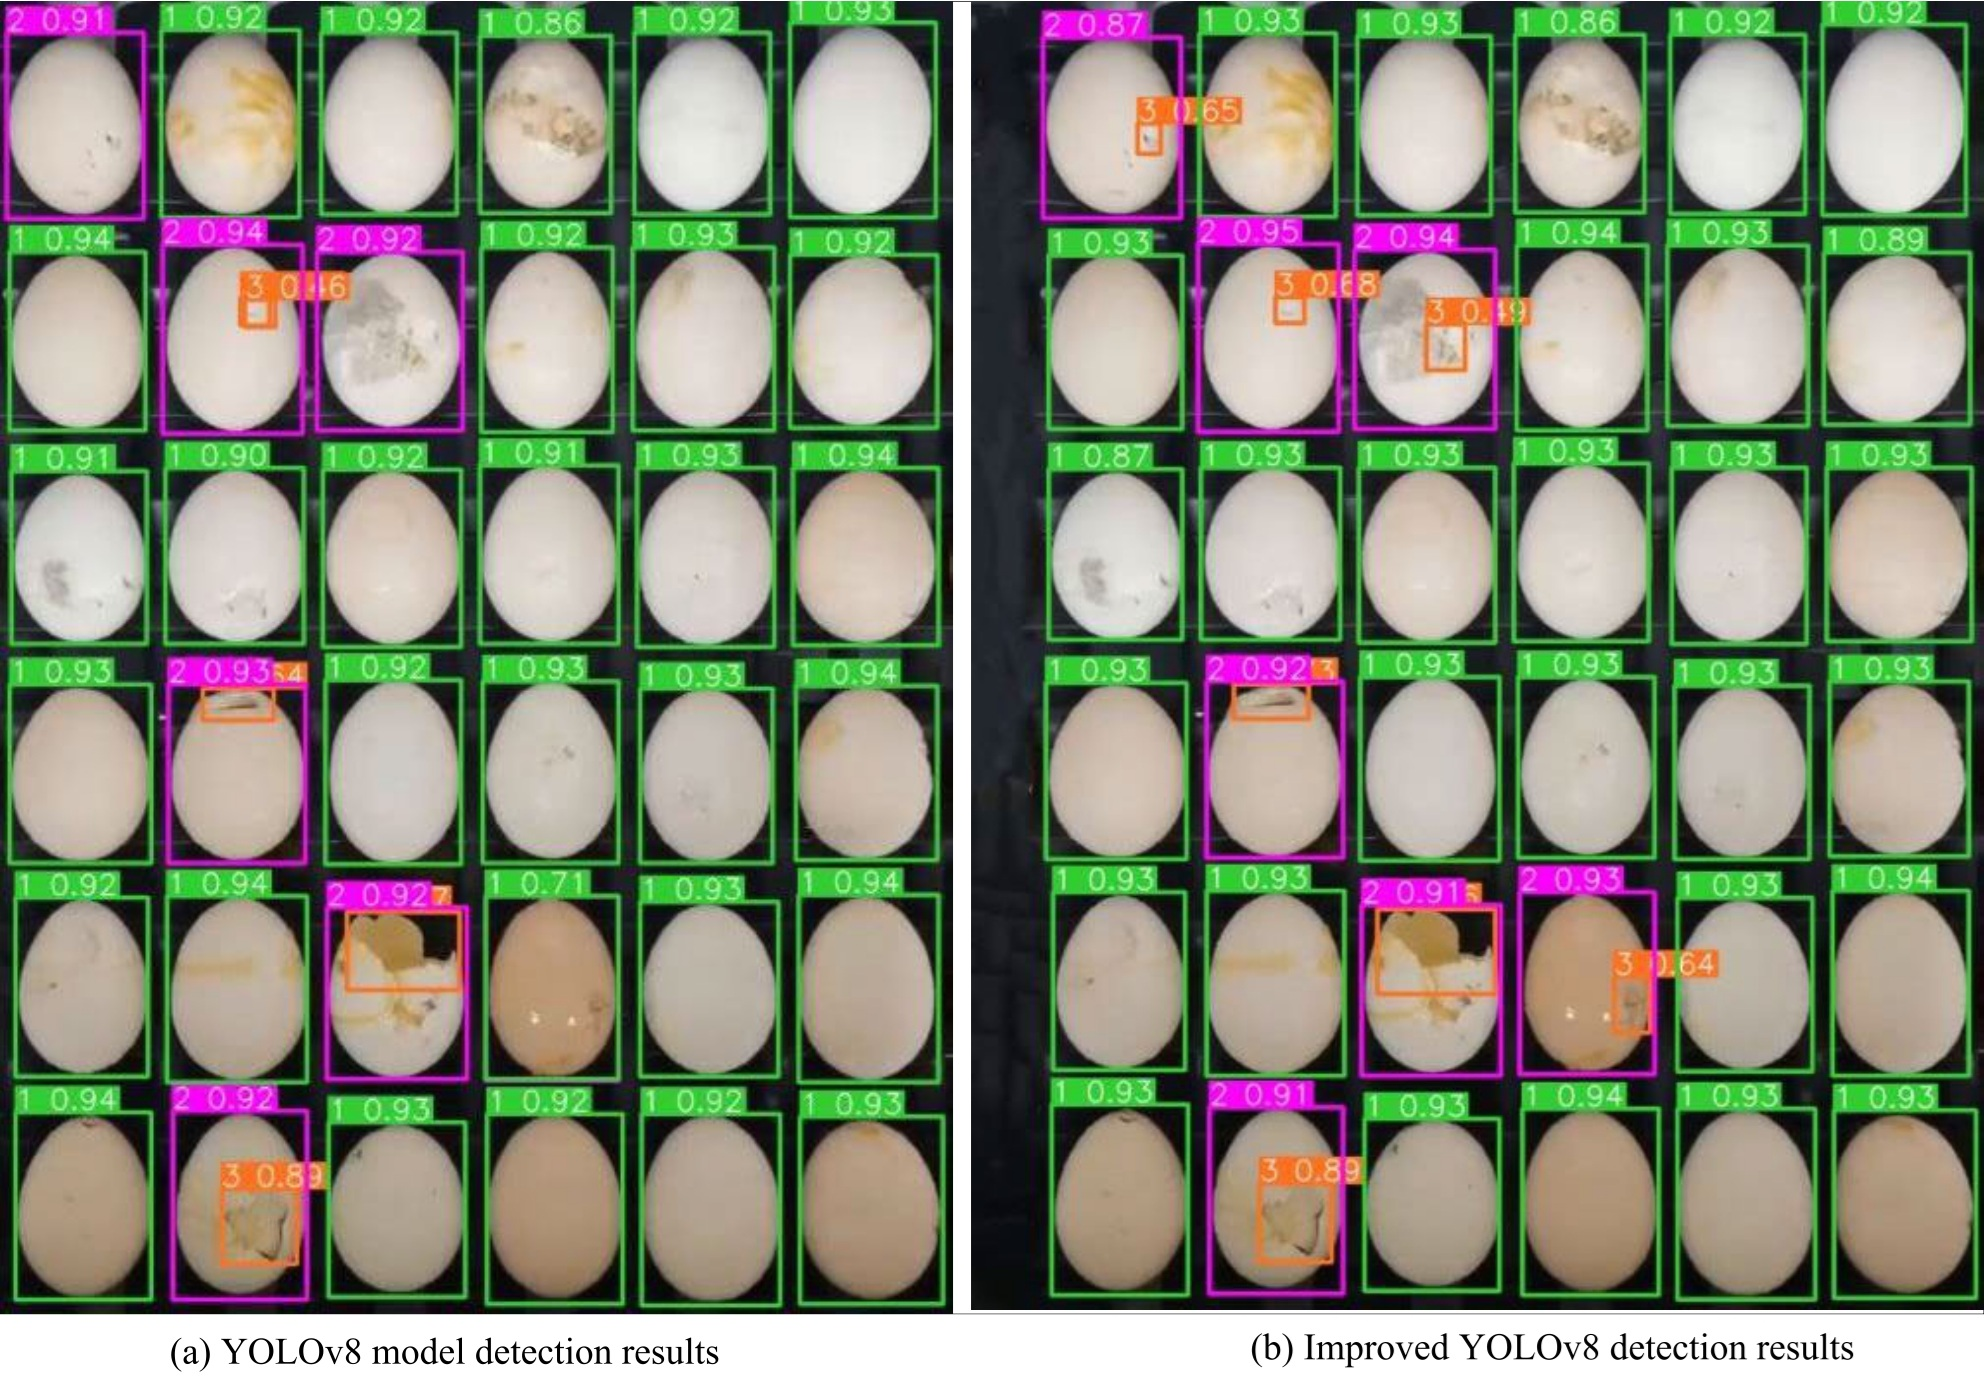
\includegraphics[width=0.80\textwidth]{figure10_production_line_detection.jpg}
    \caption{Visual detection results on active industrial conveyor with rotating eggs}
    \label{fig:production_detection}
\end{figure}

\section{Real-Time Processing Speed and Temporal Stability}

Figure~\ref{fig:online_speed} plots the frame-by-frame inference speed across 400 continuous video frames during factory online testing.

\begin{figure}[H]
    \centering
    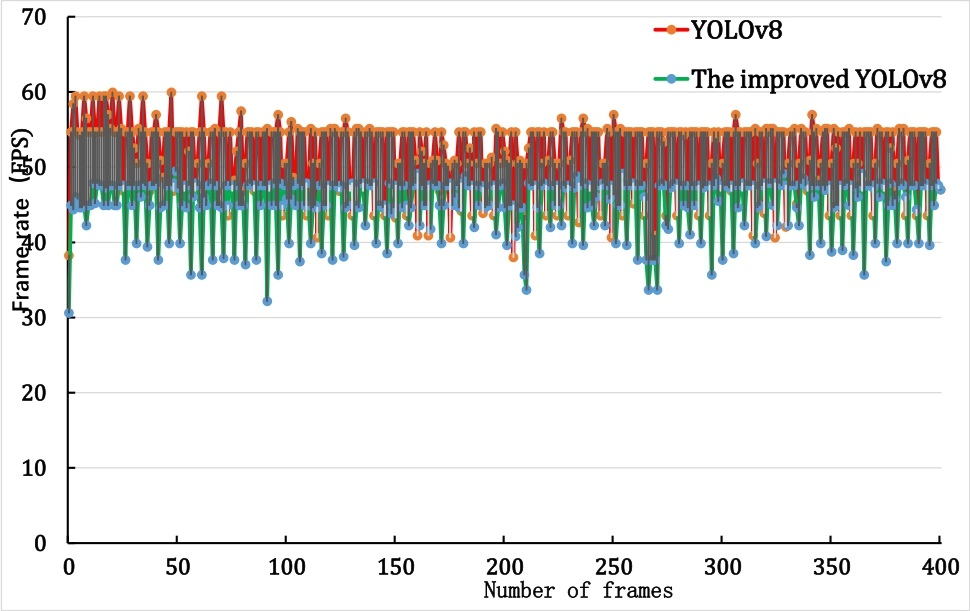
\includegraphics[width=0.75\textwidth]{figure11_online_detection_speed.jpg}
    \caption{Online detection speed stability curve across 400 continuous frames at 45 FPS}
    \label{fig:online_speed}
\end{figure}

The inference latency remains exceptionally stable, hovering tightly around 45 FPS throughout continuous operation. Although slightly lower than baseline YOLOv8 (52 FPS) due to the addition of DCNv2, BiFPN and the P2 head, 45 FPS far exceeds the required conveyor throughput rate of 30 FPS, leaving ample margin for online communication and mechanical sorting actuation.

%=========================================================
% CHAPTER 4: DISCUSSION
%=========================================================

\chapter{Discussion}

\section{Speed Versus Accuracy Trade-Off in Industrial Grading}

In automated quality grading, system utility requires striking a delicate balance between inference latency and detection precision. A high-accuracy model with excessive inference latency creates production bottlenecks, whereas an ultra-fast model with lower accuracy permits defective products to enter commercial channels.

As demonstrated in Chapter 3, the proposed improvements introduced a modest reduction in raw frame rate from 52 FPS to 45 FPS (-13.5\%). However, this computational cost yielded a substantial +5.2 percentage point gain in mAP@0.5 (from 87.7\% to 92.9\%), reduced the intact egg false alarm rate from 4.00\% to 2.18\% and achieved a compound cracked egg miss rate of only 1.06\%. Because industrial conveyor lines operate at 360 eggs per minute across six channels (equivalent to approximately 30 frames per second video throughput), operating at 45 FPS provides a comfortable 50\% computational headroom. This trade-off, accepting a minor speed reduction to secure superior detection accuracy, is well-justified for commercial poultry packaging.

\section{Adaptability to Natural Shell Surface Contaminants}

A primary failure mode of conventional computer vision systems in poultry processing is sensitivity to surface dirt. Commercial eggs are frequently sorted prior to washing. In unwashed conditions, natural surface contaminants such as feather debris, dust flecks and dried manure streaks produce sharp optical contrast boundaries that trigger false positives in gradient-based edge detectors and standard convolutional networks.

The proposed architecture resolves this challenge through the collaborative action of DCNv2 and triple classification granularity. Deformable convolution dynamically reshapes receptive field sampling patterns along continuous curvilinear crack trajectories, effectively ignoring localized, irregular dirt blotches. Furthermore, by independently supervising Category 2 (holistic cracked egg) and Category 3 (localized crack region), the network learns to decouple structural fracture morphology from superficial dirt textures, reducing the false alarm rate on intact unwashed eggs to 2.18\%.

\section{Generalization Across Diverse Poultry Egg Varieties}

In commercial production, eggshell appearance varies considerably across avian breeds and species. For eggs with uniform, solid-colored shells, such as brown hen eggs and white duck eggs, the proposed detection framework exhibits strong feature contrast. The visual indicators of shell rupture, consisting of abrupt color shifts, shadowed fracture lines and localized surface glossiness variations, provide prominent signals that the network readily identifies.

Conversely, for eggs with heavily patterned or speckled shells, such as quail eggs, defect recognition presents dual characteristics. The intricate natural pigmentation of intact quail shells creates a complex, high-frequency background that increases the risk of false alarms. However, when structural fractures occur that involve underlying albumen or yolk leakage, the distinctive wet, highly reflective optical signature of the damaged area produces a strong, unmistakable feature response. Extending training datasets across cross-species egg varieties represents a promising avenue for universal poultry grading.

\section{Technical Challenges with Reticular Micro-Cracks}

Despite the strong performance achieved by the improved YOLOv8 model, fine reticular spider-web cracks remain the most challenging defect category. These micro-cracks exhibit aperture widths below 0.03 mm and lack pronounced structural displacement. Under standard top-down diffuse LED illumination, these hairline cracks cast virtually no geometric shadow, producing faint edge gradients that blend into the natural micro-texture of the calcite crystalline matrix.

When reticular micro-cracks appear on unwashed eggs, their visual ambiguity increases further, occasionally leading to false negatives in individual video frames. Although multi-frame accumulation across the 60-frame inspection window partially compensates for weak single-frame responses, addressing this challenge at the source requires specialized optical engineering. Implementing dark-box illumination setups, where grazing-angle side lighting illuminates crack fissures via internal refraction while leaving the surrounding shell dark, presents an effective solution to enhance crack gradient contrast.

\section{Edge Computing Deployment and Industrial Hardware Integration}

Practical deployment within harsh poultry farm environments requires robust hardware integration and active environmental maintenance protocols:
\begin{itemize}
    \item \textbf{Edge Computing Platform:} With a parameter count of $2.66 \times 10^7$ and a model file size of 51.1 MB, the improved network can be deployed onto embedded edge AI accelerators such as the NVIDIA Jetson AGX Orin. Applying TensorRT FP16 quantization accelerates inference latency to under 12 ms per frame.
    \item \textbf{Pneumatic Sorting Actuation:} The machine vision software interfaces with downstream programmable logic controllers (PLCs) synchronized via optical rotary shaft encoders. When an egg is flagged as cracked, high-speed solenoid air valves trigger a calibrated 20 ms compressed air pulse, gently lifting the defective egg into an exit chute without mechanical impact damage.
    \item \textbf{Environmental Protection:} Poultry sorting facilities carry heavy airborne dust and humidity. Installing positive-pressure air knives across optical camera windows prevents airborne feather dust from settling on lenses, while thermostatically regulated LED cooling fans prevent color temperature shifts during prolonged multi-shift operations.
\end{itemize}

%=========================================================
% CHAPTER 5: CONCLUSION
%=========================================================

\chapter{Conclusion}

\section{Conclusion}

This seminar presented a comprehensive investigation of an industrial-grade, real-time cracked egg detection system combining an improved YOLOv8 deep learning architecture, multi-channel rotational conveyance and a redundant dual verification mechanism with triple classification granularity. The mechanical conveying assembly features six parallel inspection channels equipped with motor-driven rotating rollers, ensuring that each moving egg undergoes complete 360-degree axial rotation beneath an overhead industrial CCD camera and uniform LED illumination box, entirely eliminating circumferential inspection blind spots.

To address the limitations of conventional binary classification and rigid convolutional kernels, the framework established a triple classification granularity paradigm comprising Intact Egg (Category 1), Cracked Egg (Category 2) and localized Crack Region (Category 3). At the architectural level, baseline YOLOv8 was structurally optimized by embedding Deformable Convolution v2 (DCNv2) into the backbone to adapt receptive field sampling grids to irregular crack contours, replacing the PANet neck with a Weighted Bidirectional Feature Pyramid Network (BiFPN) for adaptive multi-scale feature fusion, adding a dedicated P2 small target detection head operating on a $160 \times 160$ feature map to preserve high-frequency micro-crack edges and implementing the Wise-IoU v2 (WIoUv2) dynamic loss function to dynamically balance gradient penalties across bounding box candidates.

Experimental evaluations conducted on an industrial dataset of 3,222 unwashed egg images demonstrated that the improved YOLOv8 network achieves a Mean Average Precision (mAP@0.5) of 92.9\%, representing a 5.2 percentage point improvement over baseline YOLOv8 and outperforming Faster R-CNN (78.1\%), YOLOv5 (85.2\%) and YOLOv11 (87.3\%). During live industrial deployment on an active egg conveyor line, the deployed system maintained a continuous processing throughput of 45 frames per second, reduced the intact egg false alarm rate to 2.18\% and achieved a compound cracked egg miss rate of only 1.06\% under dual verification logic, fully satisfying real-time commercial egg packaging criteria.

\section{Future Scope}

Based on the research findings and operational insights of the base paper, future investigations will focus on four specific directions:
\begin{enumerate}[label=\arabic*.]
    \item \textbf{Feature Super-Resolution and Attention Magnification:} Exploring advanced small-object detection algorithms, including feature super-resolution networks and attention-guided patch magnification mechanisms, to specifically boost edge gradient sensitivity and further reduce false negative rates on sub-millimeter damaged areas.
    \item \textbf{Expanded Multi-Variety Poultry Datasets:} Collecting and annotating extensive industrial datasets encompassing diverse mechanical damage patterns, severe impact fractures and different poultry egg varieties (including duck eggs and patterned quail eggs) to further validate and strengthen model generalization across diverse commercial packaging lines.
    \item \textbf{Dark-Box Specialized Illumination Systems:} Developing and incorporating specialized dark-box illumination setups utilizing grazing-angle lateral lighting and optical polarization to enhance the visual edge contrast of fine net-like reticular cracks against healthy shell backgrounds.
    \item \textbf{Unified Multi-Defect Inspection Frameworks:} Integrating the surface crack detection system into a broader, multi-modal poultry egg quality evaluation platform combining internal candling and near-infrared spectroscopy to achieve simultaneous, unified detection of internal defects such as scattered yolk, blood spots and bacterial spoilage alongside exterior shell cracks.
\end{enumerate}

%=========================================================
% REFERENCES
%=========================================================

\chapter*{References}
\markboth{References}{}
\addcontentsline{toc}{chapter}{References}

\begin{enumerate}[label={[\arabic*]}]

\item D. Sun, H. Wei, Y. Luo, W. Li and Y. Yu,
``Real-Time Detection Method for Cracked Eggs Based on Improved YOLOv8 and Dual Verification With Triple Classification Granularity,''
\textit{IEEE Access}, vol. 14, pp. 62322-62333, Apr. 2026, doi: 10.1109/ACCESS.2026.3686452.

\item D. Liang, P. Li, D. Liang, J. Qian and B. Li,
``Integrated detection and grading system for internal and external quality of eggs based on machine vision,''
\textit{Journal of Chinese Institute of Food Science and Technology}, vol. 20, no. 11, pp. 247-254, Nov. 2020.

\item A. Datta, B. Botta and S. Gattam,
``Damage detection on chicken eggshells using faster R-CNN,''
in \textit{Proc. ASABE Annual International Meeting}, Boston, MA, USA, Jul. 2019, p. 1244.

\item M. Turkoglu,
``Defective egg detection based on deep features and bidirectional long-short-term-memory,''
\textit{Computers and Electronics in Agriculture}, vol. 185, Jun. 2021, Art. no. 106152.

\item B. Botta, S. S. R. Gattam and A. K. Datta,
``Eggshell crack detection using deep convolutional neural networks,''
\textit{Journal of Food Engineering}, vol. 315, Feb. 2022, Art. no. 110798.

\item J. Yin, J. Kang and D. Xiao,
``Lightweight duck egg crack detection algorithm based on improved YOLOv5l,''
\textit{Transactions of the Chinese Society of Agricultural Engineering}, vol. 40, no. 1, pp. 165-173, Jan. 2024.

\item Y. Huang, Y. Luo, Y. Cao, X. Lin, H. Wei, M. Wu, X. Yang and Z. Zhao,
``Damage detection of unwashed eggs through video and deep learning,''
\textit{Foods}, vol. 12, no. 11, p. 2179, May 2023.

\item X. Zhu, H. Hu, S. Lin and J. Dai,
``Deformable ConvNets v2: More Deformable, Better Results,''
in \textit{Proc. IEEE/CVF Conference on Computer Vision and Pattern Recognition (CVPR)}, Long Beach, CA, USA, Jun. 2019, pp. 9308-9316.

\item M. Tan, R. Pang and Q. V. Le,
``EfficientDet: Scalable and Efficient Object Detection,''
in \textit{Proc. IEEE/CVF Conference on Computer Vision and Pattern Recognition (CVPR)}, Seattle, WA, USA, Jun. 2020, pp. 10778-10787.

\item Z. Tong, Y. Chen, Z. Xu and R. Yu,
``Wise-IoU: Bounding Box Regression Loss with Dynamic Focusing Mechanism,''
\textit{arXiv preprint arXiv:2301.10051}, Jan. 2023.

\item Z. Balci, I. Yabanova and A. Mert,
``An acoustic signal-to-image conversion integrated convolutional neural network model for egg crack detection,''
\textit{British Poultry Science}, vol. 67, no. 2, pp. 224-232, Mar. 2026.

\item L. Sun, S. Feng, C. Chen, X. Liu and J. Cai,
``Identification of eggshell crack for hen egg and duck egg using correlation analysis based on acoustic resonance method,''
\textit{Journal of Food Process Engineering}, vol. 43, no. 8, p. 13430, Aug. 2020.

\item A. Nasiri, M. Omid and A. Taheri-Garavand,
``An automatic sorting system for unwashed eggs using deep learning,''
\textit{Journal of Food Engineering}, vol. 283, Oct. 2020, Art. no. 110036.

\item Y. Luo, Y. Huang, Q. Wang, K. Yuan, Z. Zhao and Y. Li,
``An improved YOLOv5 model: Application to leaky eggs detection,''
\textit{LWT - Food Science and Technology}, vol. 187, Sep. 2023, Art. no. 115313.

\item J. Redmon, S. Divvala, R. Girshick and A. Farhadi,
``You only look once: Unified, real-time object detection,''
in \textit{Proc. IEEE Conference on Computer Vision and Pattern Recognition (CVPR)}, Las Vegas, NV, USA, Jun. 2016, pp. 779-788.

\end{enumerate}

\end{document}